% ========== Chapter 2
 
\chapter {\uppercase{Computational approaches to reconstruct gene regulatory networks}}
\label{chap:2}

 A challenge of systems biology has been inference of comprehensive and accurate gene regulatory networks (GRNs) directly from genome sequence and transcriptome data. In this chapter, I describe computational approaches for reverse engineering accurate GRNs from gene expression data. There are diverse approaches to the problem: from information theoretic to correlational to integrated. I focus on two algorithms that play a central role in the work described here: \cm\ \cite{reiss_integrated_2006} and \nwinf\ \cite{bonneau_inferelator:_2006}, as well as the model derived from integrating the two, the Environment and Gene Regulatory Influence Network or EGRIN \cite{bonneau_predictive_2007}. Following introduction of these components, I discuss methods developed specifically for this dissertation, an ensemble of EGRIN models. I review the history and motivation for ensemble modeling. I document all of the methods, data, and analyses used to construct models for \halo and \eco. Additionally, I provide validation for the model's predictions, as well as evaluation of its robustness. The details described in this chapter are the foundation from which I derive biological insight in the following chapters.\\

 \noindent This chapter has been modified from the supplement to: \\

 \noindent Brooks AN$^{*}$, Reiss DJ$^{*}$, Allard A, Wu W, Salvanha DM, Plaisier CL, Chandrasekaran S, Pan M, Kaur A, Baliga NS. (2014) A system-level model for the microbial regulatory genome. \emph{Mol Syst Biol.}  10: 740.\\

 \noindent * Indicates equal contribution 

 \paragraph{Chapter Highlights}

	\begin{itemize}
	\item Many algorithms for GRN inference exist. Methods vary significantly in their approach. 
	\item \cm\ integrates multiple sources of biological data, including gene expression, to identify condition-specific co-regulatory modules called biclusters
	\item \nwinf\ predicts which TFs influence condition-specific regulation of these biclusters using regression and variable selection
	\item Together, the two algorithms generate an Environment and Gene Regulatory Influence Network (EGRIN)
	\item Ensemble network inference in \egrine\ improves performance by reducing model variance and allowing detection of rare co-regulatory events 
	\item We derived biological insight from the ensemble model by applying network-based methods for backbone extraction and link community detection
	\item Extensive support for model predictions from independent experimental validation data
	\item \egrine~outperforms other GRN inference methods 
	\end{itemize}

\section{Summary}

Many methods exist for reconstructing GRNs from transcriptomic data. Integrating additional supporting data can assist network reconstruction. \cm\ is a stochastic semi-supervised machine learning algorithm for inferring GRNs that uses \textit{cis}-regulatory motif detection and biological support in known functional networks to constrain model selection. \nwinf~predicts influence of TFs on the expression of \cm~biclusters. Running \cm\ and \nwinf~in an ensemble framework greatly improves performance. The resulting \egrine\ model is more accurate and reveals genetic mechanisms through which bacteria reuse gene modules across diverse environments to enhance fitness.  

\section{Existing computational approaches}

There are many approaches to GRN inference. So many, in fact, that entire reviews have been written about them \cite{bansal_how_2007,de_smet_advantages_2010}. There has even been a formal competition between algorithms. While full description of all approaches is outside the scope of this manuscript, I briefly cover some of the more popular methods, especially those that factor into the present study. 

Methods for GRN inference vary significantly in their fundamental approach to the problem. While each tries to infer an accurate and comprehensive GRN directly from gene expression data, many of the methods take fundamentally different approaches. Some methods use regression (e.g., \nwinf\ described extensively below), some correlation (e.g. WGCNA); some are information based (e.g., CLR and ARACNE), whereas others are Bayesian; others still are integrated, using additional data to perform inference (e.g., \cm) or use other methods entirely (e.g. Genie3 \cite{huynh-thu_inferring_2010}).Newer methods, including our own and DREAM5, aggregate across multiple runs of the same algorithm (e.g. \egrine, the method developed here) or integrate across multiple, heterogeneous methods (e.g, DREAM5).

\paragraph{CLR} Context likelihood of relatedness, CLR \cite{faith_large-scale_2007}, is a mutual information based approach that builds on relevance networks \cite{eisen_cluster_1998,butte_mutual_2000}. CLR (like relevance networks) calculates mutual information between each TF and every gene in the genome using mutual information (MI), where mutual information is a measure of the statistical dependence between two variables. The resulting network can be cut at some threshold MI value to produce a GRN (only TF$\rightarrow$gene above the threshold are retained). CLR adds to relevance networks by introducing an adaptive background correction step that tries to assess how significant each TF$\rightarrow$gene MI value is in the context of every other possible interaction for either that TF or gene. Only those that MI values that are statistically distinguishable from background are retained.  This step is designed to remove indirect dependencies in the network to retain only direct TF$\rightarrow$gene interactions. 

\paragraph{ARACNE} ARACNE is also an information theoretic approach to reconstructing GRNs \cite{margolin_aracne:_2006}. It uses MI to infer TF$\rightarrow$gene interactions as well. Unlike CLR, it uses the data processing inequality (DPI) to remove indirect dependencies. DPI removes the lowest MI from every every gene triplet in network above a certain threshold. The basic idea is that direct interactions will have a higher MI. Thus in the following three gene scenario: $A \rightarrow B \rightarrow C$, $MI_{A,C} < MI_{B,C}$.

\paragraph{WGCNA} Weighted gene correlation network analysis, WGCNA, computes pairwise correlation (weighted or unweighted) between every pair of genes followed by hierarchical clustering and dynamic tree cut to define gene co-expression modules \cite{langfelder_wgcna:_2008}. Unlike ARACNE and CLR, WGCNA does not specifically predict TF$\rightarrow$gene interaction, rather it produces gene co-expression modules (like the \cm\ component of EGRIN, described below).

\paragraph{DISTILLER} DISTILLER, like \cm, produces biclusters (sets of gene co-expressed in subsets of the experiments) by integrating gene expression data with interaction data from RegulonDB \cite{lemmens_distiller:_2009}. DISTILLER is one of the algorithms we compare our method against (given their similarities). We obtained \textit{E. coli} expression data from this paper. 

\paragraph{DREAM5} Dialogue for Reverse Engineering Assessments and Methods (DREAM) is an annual competition for computational methods. In 2012, a group running the competition made a community network of all the top scoring entries for a GRN inference challenge. As described below, this is a type of ensemble model (similar in spirit to our own). The group integrated the predictions from various methods using Borda count election method. Basically, they retained the TF$\rightarrow$gene predicted by the most algorithms. 

\paragraph{EGRIN} Environment and Gene Regulatory Influence Network (EGRIN) uses biclustering in addition to regression and variable selection to infer both gene modules (biclusters) and specific TF$\rightarrow$gene influences \cite{bonneau_predictive_2007}. The approach consists of the algorithms \cm\ \cite{reiss_integrated_2006} and \nwinf\ \cite{bonneau_inferelator:_2006}. Since these algorithms are the basis for this dissertation work, they will be described in great detail below. \\

\noindent A comprehensive review of available methods and comparison between them is available in \cite{de_smet_advantages_2010} and the supplement to \cite{marbach_wisdom_2012}.

\subsection{Integrated biclustering using \cm}

\label{chap:2:cmonkey}

\subsubsection{\cm\ introduction}

The \cm\ integrated biclustering algorithm was described and fully benchmarked in \cite{reiss_integrated_2006}. In short, the algorithm computes putatively co-regulated modules of genes over subsets of experimental conditions from gene expression data, constrained by information provided by genome sequence (\textit{de novo} identification of conserved \textit{cis}-regulatory motifs in gene promoters), and functional association networks. Its defining characteristic is that it combines all three types of data (expression, sequence and networks)together into an integrated model that uses a stochastic optimization procedure to identify modules that best satisfy all three constraints, simultaneously.

The \cm\ integrated biclustering algorithm identifies groups of genes co-regulated under subsets of experimental conditions, by integrating various orthogonal pieces of information that support evidence for their co-regulation, and optimizing biclusters such that they are supported by one or more of those additional constraints. The three sources of evidence for co-regulation leveraged by \cm\ to score gene clusters are (1) tight co-expression in subsets of available gene expression measurements (similarity of expression profiles); (2) quality of \textit{de novo} detected \textit{cis}-regulatory motifs in gene promoters (putative co-binding of common regulators); and (3) significant connectivity in functional association or physical interaction networks (co-functionality). The algorithm served as the cornerstone for the construction of the first global, predictive Environmental Gene Regulatory Influence Network (EGRIN) model for \halo\ \cite{bonneau_predictive_2007}, and has now been applied to many additional organisms (\eg, \cite{yoon_systems_2013} and unpublished).

To run \cm\ as part of an ensemble-based inference approach required significant updates to the \cm\ algorithm. These updates primarily addressed computational inefficiencies that led to long runtime. The primary algorithm modification in the new implementation is global optimization (rather than the local, individual cluster optimization utilized by the original procedure). Additional algorithm updates include changes to the individual scoring scheme for subnetwork clustering, as well as integration of the scores. All of these changes improved the procedure's runtime without significantly affecting the algorithm's performance.

\begin{figure}[h!]
\centering
\includegraphics[width=0.9\linewidth]{figures/bicluster}
\caption[Bicluster: a conditionally co-regulated module]{\cm\ produces a set of biclusters ($\sim$300), each of which consists of a group of genes that are co-regulated in some (but not all) of the experiments. Typical \cm\ bicluster is shown here. Top-left: Standardized gene expression values for each gene in the bicluster. Vertical red line separates conditions that have been excluded from the bicluster. Top-right contains an expanded view of only the conditions in which the genes are co-expressed. \cm\ also uses \textit{de novo} motif detection to support bicluster assignment. Upstream regions of bicluster genes are searched for shared \textit{cis}-regulatory motif by MEME \cite{bailey_fitting_1994}. Similarity of the genes in annotated functional networks (e.g. STRING \cite{szklarczyk_string_2011}) is also scored. Detected motif and string network shown at bottom-left. Location of the motif in gene promoters shown bottom-right.}
\label{fig:bicluster}
\end{figure}

\subsubsection{Detailed \cm\ algorithm description}

The \cm\ algorithm initiates by seeding $k$ biclusters, typically using the simple, widely-used and effective $k$-means clustering on the input expression data set. \cm\ itself performs a global optimization, in many ways similar to the $k$-means clustering algorithm, which we used as a model. After beginning with an initial assignment of each gene into $k$ clusters and a chosen distance metric, the basic$k$-means algorithm iterates between two steps until convergence: (1) (re-)assign each gene to the cluster with the closest centroid and (2) update the centroids of each modified cluster. The updated \cm\ algorithm performs an analogous set of moves with four primary distinctions: (1) the distance of each gene to the ``centroid'' of each cluster is computed using a measure that combines condition-specific expression profile similarity, $cis$-regulatory motif similarity, and connectedness in one or more gene association networks; (2) each gene can be (re-)assigned to more than one cluster (default 2); (3) at each step, conditions (in addition to genes) are moved among biclusters to improve their cohesiveness; and (4) at each step, genes and conditions are not always assigned to the most appropriate clusters. We now elaborate upon these four details.

\cm\ begins each iteration with a set of bicluster memberships $\{m_i\}$ for each element (gene or condition) $i$, where by default $\|m_i\| = 2$ for genes and $\|m_i\| = N_c/2$ for conditions ($N_c$ is the number of conditions, or measurements, in the expression data set; note that for standard $k$-means clustering, $\|m_i\| = 1$ for genes and $\|m_i\| = N_c$ for conditions). \cm\ then computes score matrices (log-likelihoods, in practice) $\mathbf{R}_{ij}$, $\mathbf{S}_{ij}$, and $\mathbf{T}_{ij}$, for membership of each element $i$ in each bicluster $j$, based upon, respectively, co-expression with the current gene members ($\mathbf{R}$), similarity of motifs in gene promoters ($\mathbf{S}$), and connectivity of genes in networks ($\mathbf{T}$). For the network scores ($\mathbf{T}$), the originally published procedure \cite{reiss_integrated_2006} computed a $p$-value for enrichment of network edges among genes in each bicluster using the cumulative hypergeometric distribution. This computation was inefficient, and moreover could not account for weighted edges in the input networks, so we replaced it with a more standard weighted network clustering coefficient \cite{watts_collective_1998}, evaluated only over the genes within each bicluster.

Following computation of the individual component scores, \cm\ computes a score matrix $\mathbf{M}_{ij}$ containing the integrated score (a weighted sum of log-likelihoods) supporting the inclusion of gene $i$ in bicluster $j$. At this stage the updated version of \cm\ then computes a cumulative density distribution from each bicluster's $\mathbf{M}_{\cdot j}$ to obtain a posterior probability distribution $p_{ij}$, that each element $i$ should be in each cluster $j$, which is used to classify cluster members based upon these scores. The width of the density distribution kernel is set dynamically to be larger for smaller (fewer gene) biclusters, so as to increase the tendency to add genes to small biclusters, rather than to remove them. In the updated procedure, we then add a small amount of normally-distributed random ``noise:'' to the scores $\mathbf{M}_{ij}$, in order to achieve a similar type of stochasticity to the original version of the algorithm (which was originally obtained using sampling, and which helps prevent the algorithm from falling into local minima; this noise decreases during the run to zero at the final iteration). The result of this noise is that at the beginning of a \cm\ run, biclusters are rather poorly defined (co-expression, for example, is weak), but during the course of a full set of 2,000 iterations, as this noise is decreased, the biclusters settle into minima.

Finally, at the end of each iteration, \cm\ chooses a random subset of elements (genes or conditions) $i$, and moves $i$ into bicluster $j$ if, for any biclusters $j'$ which it is already a member, $p_{ij} > p_{ij'}, \forall j'$, and out of the corresponding worse bicluster $j'$ for which $p_{ij} > p_{ij'}$. Thus, as with the $k$-means clustering algorithm, the updated \cm\ performs a global optimization of all biclusters by moving elements among biclusters to improve each element's membership scores.

\subsubsection{\cm\ software availability}

The \cm\ software is available as an open-source \tmsamp{R} package \cite{ihaka_r:_1996}.  With this package the algorithm can be easily applied to nearly any sequenced microbial species (given user-supplied expression data). The package automatically downloads and integrates genome and annotation data from various external sources, including \tmsamp{RSA-tools} \cite{van_helden_web_2000}; \tmsamp{Microbes Online} \cite{alm_microbesonline_2005}; and \tmsamp{EMBL STRING} \cite{szklarczyk_string_2011}. Additionally, the package can generate interactive web-based and \tmsamp{Cytoscape} output \cite{shannon_cytoscape:_2003}, allowing users to explore the resulting modules and motifs in the context of external data, software, and databases via the \tmsamp{Gaggle} \cite{shannon_gaggle:_2006}. Examples of automatically generated output are available at the \cm\ web site. Supplementary $R$ packages with example expression data for organisms including \halo\ and \eco\ are also available from the \cm\ website.

\subsection{Assignment of putative regulators and influence using \nwinf}

\subsubsection{\nwinf\ introduction}

The \nwinf\ algorithm is a method for deriving genome-wide transcriptional regulatory interactions from mRNA expression levels \cite{bonneau_inferelator:_2006}. \nwinf\ is a direct inference procedure \cite{michoel_comparative_2009}. It models transcriptional regulation as a kinetic process, incorporating time information, when available, and a user-defined time constant. \nwinf\ uses standard regression and variable selection to identify transcriptional influences on genes or biclusters based on their mean expression levels. These influences include expression levels of TFs, environmental factors, and interactions between the two. The procedure simultaneously models equilibrium and time course expression levels. Thus both kinetic and equilibrium expression levels may be predicted by the resulting models. Through explicit inclusion of time and gene knockout information, the method is capable of learning causal relationships. The inferred network is a predictive model comprised of linear combinations of expression profiles of various transcriptional regulators, that can predict global expression under novel perturbations with predictive power similar to that seen over training data \cite{bonneau_inferelator:_2006}.

\subsubsection{Detailed \nwinf\ algorithm description}

Given an input list of $p$ putative transcriptional influences $\mathbf{X}={x_1,x_2,\cdots,x_p}$ and the mean expression levels $y_{i}$ of a bicluster $k$ (over the conditions $i$ included in the bicluster), we model the relationship between $y_{i}$ and the influences $\mathbf{X}$ by the kinetic equation:

\begin{equation}
\label{eq:nwinf:kinetic}
\tau\frac{dy_{i}}{dt}=-y_{i}+\sum_{j=1}^{p}\beta_j x_{ij} .
\end{equation}

\noindent In the steady state scenario, $dy/dt=0$ and Eq.~\ref{eq:nwinf:kinetic} simplifies to

\begin{equation*}
y_{i}=\sum_{j=1}^{p}\beta_j x_{ij} ,
\end{equation*}

\noindent and for time series measurements, we approximate Eq.\ref{eq:nwinf:kinetic} as:

\begin{equation*}
\tau\frac{y_{i+1}-y_{i}}{t_{i+1}-t_i} + y_{i} = \sum_{j=1}^{p}\beta_j x_{ij} .
\end{equation*}

\noindent Clearly not all $p$ putative influences $\mathbf{X}$ influence a given bicluster, so we use the elastic-net \cite{zou_regularization_2005} for variable selection. This involves performing the minimization:

\begin{equation}
\label{eq:elnet}
 \vec{\beta} = \arg \min \left\{ \sum^N_{i = 1} \left( y_i - \sum^p_{j = 1} \beta_j x_{ij} \right)^2 + \sum_{j = 1}^p
   \tmmathbf{w}_i ( \lambda_1 | \beta_j | + \lambda_2 \beta^2_j) \right\}
\end{equation}

\noindent subject to a constraint which is a tuneable combination of the $L_1$ (LASSO) and $L_2$ (Ridge) regression constraints:

\vspace{-0.4in}

\begin{eqnarray*}
\label{eq:elnet:constraint}
\sum_{j = 1}^p | \beta_j | \leq \lambda_1 | \beta_{\tmop{ols}} | & & \mathrm{(}L_1\ \mathrm{constraint)}, \\
\sum_{j = 1}^p \beta^2_j \leq \lambda_2 \beta^2_{\tmop{ols}}     & & \mathrm{(}L_2\ \mathrm{constraint)}.
\end{eqnarray*}

\noindent The $w_i$ in Eq.~\ref{eq:elnet} allow different variables ($\beta$'s, in this case) to be selectively constrained. For this work, we set all $w_i=1$, \ie, no differential constraints. Redefining the constraint, such that:

\begin{equation}
\label{eq:elnet2}
 \vec{\beta} = \arg \min \left\{ \sum^N_{i = 1} \left( y_i - \sum^p_{j = 1} \beta_j x_{ij} \right)^2 + \sum_{j = 1}^p
   \tmmathbf{w}_i \lambda \left( \alpha | \beta_j | + (1-\alpha) \beta^2_j /2\right) \right\}
\end{equation}

\noindent defines $0\leq \alpha \leq 1$ as a tuning parameter between the ridge ($L_2$; $\alpha=0$) and LASSO ($L_1$; $\alpha=1)$ solutions, and $\lambda$ is the single complexity parameter, which is chosen to minimize the cross-validation error (we use 10-fold cross-validation), exactly as in \cite{bonneau_inferelator:_2006}. Substituting Eq.~\ref{eq:nwinf:kinetic} into Eq.~\ref{eq:elnet2}, we obtain the complete equation describing the minimization performed by \nwinf:

\begin{equation}
\label{eq:elnet3}
 \vec{\beta} = \arg \min \left\{ \sum^N_{i = 1} 
 \left( \tau\frac{y_{i+1}-y_{i}}{t_{i+1}-t_i} + y_{i}- \sum_{j=1}^{p} \beta_j x_{i,j} \right)^2 + \sum_{j = 1}^p
   \tmmathbf{w}_i \lambda \left( \alpha | \beta_j | + (1-\alpha) \beta^2_j /2\right) \right\}.
\end{equation}

\noindent For the current implementation, we set $\tau=10$ minutes for all TFs, and $\alpha=0.8$ for all biclusters. In the future, we could choose $\tau$ and/or $\alpha$ by cross-validation as well. When $\alpha=0$, there is no constraint, and we get the ordinary least-squares (OLS) solution with all $\beta$s non-zero. With $\alpha=1$, we select the null model. The optimal solution is somewhere in-between, and this is usually the selected solution for each bicluster, usually $\sim 6$ TFs, on average; although the null model (no solution) is selected for a number of biclusters.

\subsection{Ensemble methods to decrease model variance}

Ensemble methods have become increasingly popular in statistical machine learning. The primary reason for their popularity is the observation that combining predictions reduces model variance, i.e. by combining predictions across multiple models, one can produce an aggregate model that is usually more accurate than the best of its components \cite{seni_ensemble_2010}. For most data-driven problems, there are many possible computational approaches. Ahead of time one may not know (or have some way to determine) the method that will perform best on the data. By combing predictions into an ensemble, one can guarantee that the aggregate model will perform better than most individual methods. While it may not always outperform the best method, the aggregate model will perform better than the worst approach. This is especially useful when convenient benchmarks do not exist to evaluate model performance (to, for example, identify which methods is performs worst). 

Ensemble methods gained popularity during the Netflix Prize. Netflix offered 1,000,000 dollars to anyone who could improve their internal movie recommendation system by 10\%. In the end, best performance was obtained by weighing predictions from the top 30 methods \cite{seni_ensemble_2010}. A similar approach was recently taken to infer gene regulatory networks. Multiple investigators submitted algorithms to a competition called DREAM5. The competition organizers collated these into a ``wisdom of the crowds'' community network that performed better than most (but not all) methods on multiple data sets \cite{marbach_wisdom_2012}. 

Some examples of well-known ensemble approaches for single algorithms include bagging \cite{breiman_bagging_1996}, random forests \cite{breiman_random_2001}, AdaBoost \cite{freund_desicion-theoretic_1995}, and GradientBoosting \cite{friedman_greedy_????}. We note that methods for single algorithm ensembles is different than heterogeneous ensembles, although the motivations are similar.  
The approach we took for \egrine\ is similar to bagging, i.e. bootstrap aggregation \cite{breiman_bagging_1996}. In the following sections, we detail construction of the \egrine\ ensemble. 

\section{\egrine}

\subsection{Background and motivation}

The procedure to infer a single global Environment and Gene Regulatory Influence Network (EGRIN) model from genome-wide data was described previously \cite{bonneau_predictive_2007,bonneau_inferelator:_2006,reiss_integrated_2006}. In short, the two-step procedure involves running \cm~once to obtain a single set of $\sim 300$ biclusters of genes. Genes in these biclusters have tight co-expression over a subset of the measured conditions (usually about half), are supported by common putative \textit{cis}-regulatory motif(s) in their promoters (gene regulatory elements, GREs), and are often substantiated by high connectivity in functional association networks. Next, given a set of ``predictors'' (mRNA expression levels of transcription factors and/or quantitative values for environmental factors; \eg, concentrations, growth media, etc.), and the mean expression levels of genes in each bicluster, \nwinf~is run to choose a parsimonious subset of those predictors that can accurately predict the expression levels of that bicluster (\ie., those with non-zero $\beta$ [Eq~\ref{eq:elnet3}]) . Predictors are selected independently for each bicluster. The combined set of TF$\rightarrow$bicluster interactions and their associated weights ($\beta$s) give the degree of activation (or repression) predicted.

The \egrine~modeling procedure updates this process by applying updated \cm\ and \nwinf\ algorithms (described above) repeatedly to subsets of the available expression data. The end result is an ensemble of EGRIN models, each model containing biclusters and their predicted regulators, tuned to a relatively small subset of the overall input expression compendium. The experimental subsets were selected semi-randomly, with available biological information constraining the selection procedure (\ie., including whole groups of related experiments when one was randomly selected). For {\it H. salinarum}, we used manually curated metadata about each experiment to group related experiments. Since we did not have sufficient metadata from the public \textit{E. coli} data set, we grouped the conditions based upon individual experiments instead (\eg, time series).

The \egrine~inference methodology is an ensemble learning approach, more specifically a form of bootstrap aggregation \cite{breiman_bagging_1996}, or sub-bagging. Advantages of sub-bagging include simplicity (\ie, basic model averaging), reduced model variance compared to individual runs \cite{bhlmann_analyzing_2002}, and avoidance of overfitting \cite{krogh_statistical_1997}. The power of ensemble learning approaches stems from their ability to average out errors in individual models. For EGRIN models, this feature helps overcome artifacts due to both experimental and algorithmic noise. Incorrect classification in a single model that are not the result of systematic error will re-occur infrequently in subsequent runs. Similarly, overfitting is mitigated by training each individual model on a small subset of the available data. Only consistently re-discovered relationships are considered significant.

Sub-bagging of experimental conditions further allows the model to effectively up-weight a restricted set of conditions for each individual EGRIN model in the ensemble. This forces each EGRIN to model regulatory behaviors present within a more narrow range of conditions. As a result, the individual EGRIN models have the opportunity to discover features that may distinguish highly related responses or occur in a very limited number of conditions in the data set (\eg, conditions, genes, GREs).

To quantify this assumption, we constructed a separate ensemble of 30 EGRIN models trained on the complete {\it H. salinarum} data set (\ie, 1,495 conditions; no sub-setting performed). We asked how often we would discover a GRE corresponding to the well-characterized anoxic \textit{H. salinarum} TF, Bat.  Given frequent detection of the Bat GRE in our full ensemble, we expected to detect $\sim 20$ instances of the Bat GRE in the new ensemble (\ie, motifs similar to GRE \#22; Figure \ref{fig:gre_clustering} \cite{baliga_genomic_2001}). Surprisingly, we did not detect a single GRE matching Bat when all conditions were used for training (data not shown).  This is likely because the anoxic conditions in which Bat is active represents only a small portion of the entire data set.

Ensemble-based approaches are being used more frequently in biological data analyses, including random forests (\ie, bags of decision trees) \cite{breiman_bagging_1996}, and the recently-published DREAM5 community ensemble of regulatory network predictions \cite{marbach_wisdom_2012}, which we used as a benchmark in this manuscript to evaluate \egrine\ predictions for \eco. Moreover, in principle, our approach is similar to the stochastic \tmsamp{LeMoNe} algorithm \cite{joshi_module_2009}, which uses Gibbs sampling to learn ensembles of regulatory modules from gene expression data. \egrine~is distinguished from \tmsamp{LeMoNe} and similar algorithms by its ability to predict transcriptional control mechanisms (\ie, GREs) and the conditions in which they operate, both globally and within individual gene promoters.

To construct and mine the \egrine~ensemble we utilized additional model aggregation and compilation procedures, including (1) motif clustering \cite{van_dongen_using_2012} and scanning \cite{bailey_methods_1998} (Section \ref{section:gres}); (2) gene co-regulation network construction and backbone extraction \cite{serrano_extracting_2009} (Section \ref{section:gBg}); and (3) network community detection \cite{ahn_link_2010} (Section \ref{section:linkcommunity}). These methods were used to identify GREs and their genome-wide locations, gene-gene co-regulatory associations, and corems, respectively. Each of these procedures is described in more detail below. A comprehensive workflow is provided in Figure \ref{fig:workflow}.

\begin{figure}[h!]
\centering
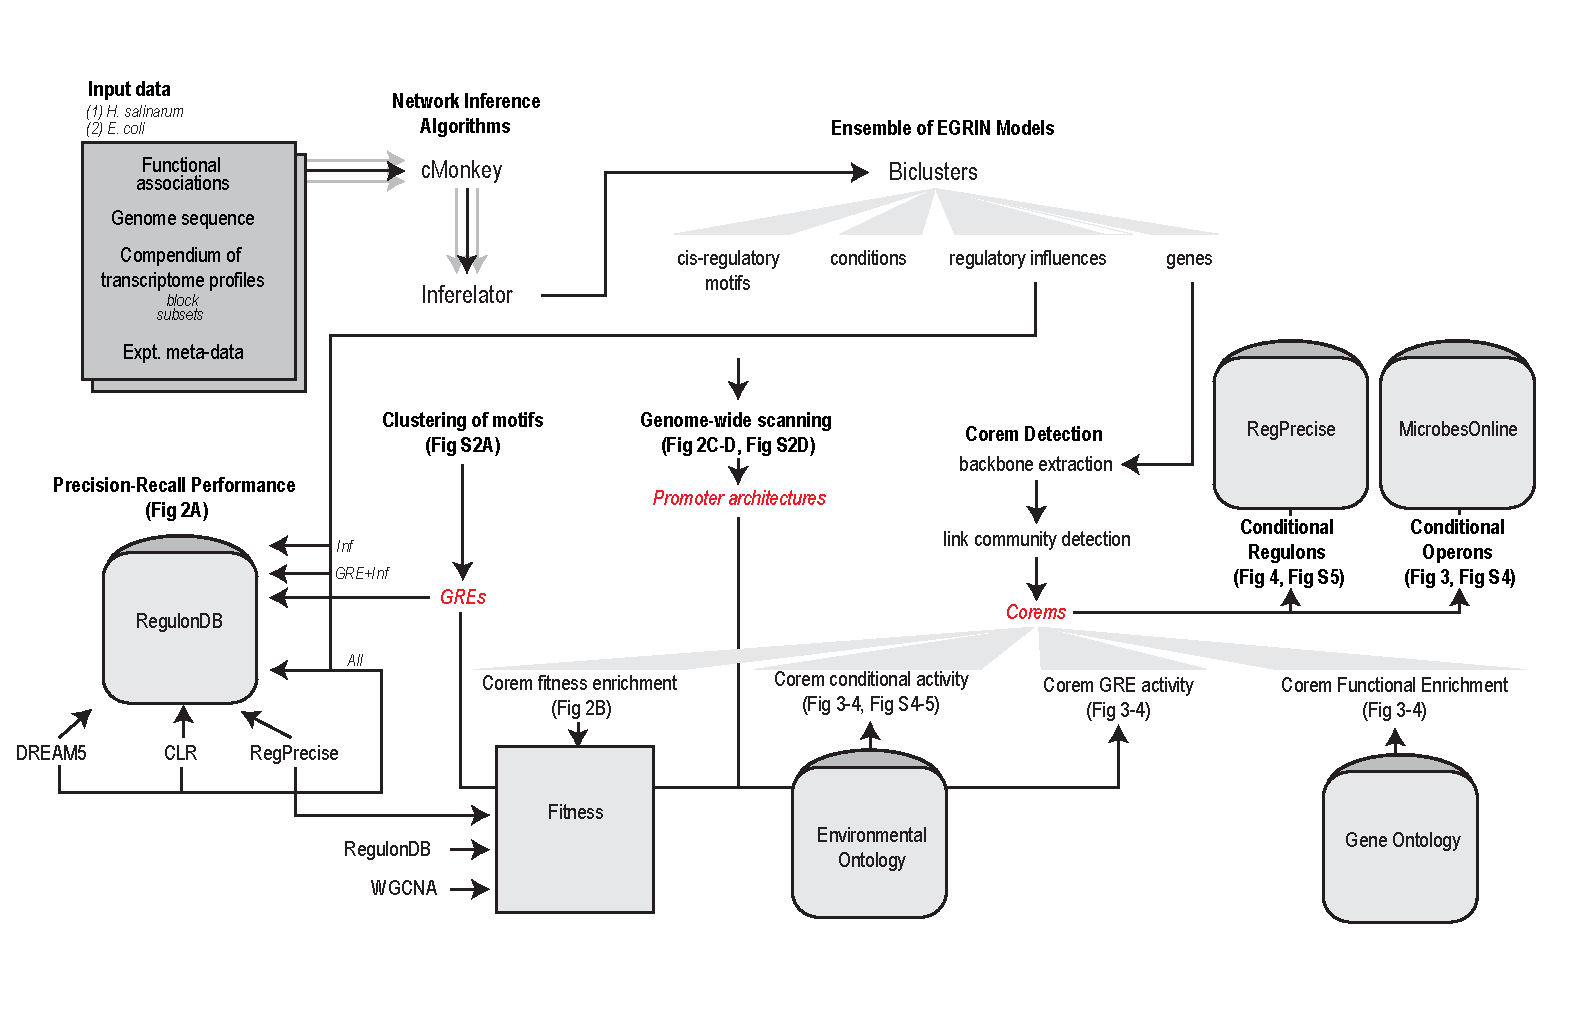
\includegraphics[width=\linewidth]{figures/workflow.pdf}
\caption[Detailed workflow for \egrine~inference procedure]{
{\bf Detailed workflow for \egrine~inference procedure.} Data input, processing and analysis to construct \egrine~model for {\it H. salinarum} and {\it E. coli}, and predictions generated. Predictions highlighted in individual figures are noted}\label{fig:workflow}
\end{figure}

% Table generated by Excel2LaTeX from sheet 'Table S2'
\begin{table}[htbp]
  \raggedright
    \begin{tabular}{|l|c|c|}
    \hline
    \textbf{Statistic} & \textit{\textbf{H. salinarum}} & \textit{\textbf{E. coli}} \\
    \hline
    %\midrule
    Arrays analyzed & 1495  & 868 \\
    Genes/transcripts & 2400  & 4213 \\
    Number of EGRIN models constructed & 572   & 106 \\
    Number of cMonkey biclusters & 142600 & 46520 \\
    Fraction of "good" cMonkey biclusters & 61\%  & 43\% \\
    Residual cutoff defining "good" biclusters & 0.40  & 0.55 \\
    Number of genes/transcripts in $\leq$ 1000 "good" biclusters (Hal) & 2104  &  \\
    Number of genes/transcripts in $\leq$ 200 "good" biclusters (Eco) &       & 4201 \\
    Average number of biclusters per gene & 1210  & 212 \\
    Number of motifs (total) & 269770 & 86167 \\
    Number of motifs (E-value $\leq$ 1) & 118546 & 15588 \\
    Number of motifs  (E-value $\leq$ 1e-6) & 32739 & 3506 \\
    Number of motif clusters & 162   & 402 \\
    Number of motifs contained in motif clusters & 37713 & 13519 \\
    Number of unique GREs & 135   & 337 \\
    Number of motifs in unique GREs & 27991 & 12773 \\
    Number of RegulonDB GREs detected (p $\leq$ 0.01) &       & 53 \\
    RegulonDB TFs with $\geq$ 3 experimentally characterized binding sites &       & 86 \\
    Corems & 679   & 590 \\
    Genes modeled by corems & 1363  & 1572 \\
    Genes per corem: min(max) & 3(377) & 3(153) \\
    Active conditions per corem: min(max) & 21(1279) & 69(598) \\
    GREs per corem: min(max) & 0(9)  & 0(12) \\
    Co-regulatory associations: prior to backbone extraction & 1573836 & 3094954 \\
    Co-regulatory associations: after backbone extraction & 141850 & 170723 \\
    Co-regulatory associations: corems & 56738 & 25976 \\
    \hline
    \end{tabular}%
    \caption{ Global properties of \textit{H. salinarum} and \textit{E. coli} ensembles}
  \label{tab:stats}%
\end{table}%

\subsection{Experimental Data}

\subsubsection{\halo~compendium}\label{halodata}

A compendium of 1495 transcriptome profiles were collated from a wide array of experiments conducted by our lab over the past decade that cover dynamic transcriptional responses to varied growth (1159 arrays), nutritional (161 arrays), and stress conditions (1102 arrays), including variation in temperature (256 arrays), oxygen (285 arrays), light (786 arrays), salinity (20 arrays), metal ions (274 arrays), and genetic perturbations (643 arrays).  We categorized the experiments using extensive metadata collected at the time of the experiment. We used this metadata to construct a GO-like ontology of the relationships between all experiments (discussed in detail below). The annotation counts above are derived from this resource (note that a single array can receive more than one annotation).  A full list of the metadata, annotations, and ontology is available on the web service.  1159 of the arrays are published (\cite{baliga_genome_2004,baliga_coordinate_2002,bonneau_predictive_2007,facciotti_large_2010,facciotti_general_2007,kaur_systems_2006,kaur_coordination_2010,schmid_two_2011,schmid_anatomy_2007,schmid_single_2009,whitehead_integrated_2006,whitehead_diurnally_2009}. 336 of the arrays are new for this study. Experimental protocols are identical to \cite{bonneau_predictive_2007}. These data, including expression levels (log$_2$ ratios vs. reference samples) and experimental metadata, are available online as a tab-delimited spreadsheet.

Each array in the {\it H. salinarum} compendium was collected using the same platform, using the same reference, and processed and normalized using the same protocol. More specifically, each RNA sample was hybridized along with a {\it H. salinarum NRC-1} reference RNA prepared under standard conditions (mid-logarithmic phase batch cultures grown at 37$^{\circ}$C in CM, OD = 0.5). Samples were hybridized to a 70-mer oligonucleotide array containing the 2400 non-redundant open reading frames (ORFs) of the {\it H. salinarum NRC-1} genome as described in \cite{baliga_genome_2004}. Each ORF was spotted on each array in quadruplicate and dye flipping was conducted (to rule out bias in dye incorporation) for all samples, yielding eight technical replicates per gene per sample. At least two independent biological replicates exist for all experimental conditions for a total of 16 replicates per gene per condition. Direct RNA labeling, slide hybridization, and washing protocols were performed as described by \cite{facciotti_general_2007,schmid_anatomy_2007}. Raw intensity signals from each slide were processed by the SBEAMS-microarray pipeline \cite{marzolf_sbeams-microarray:_2006} (www.SBEAMS.org/microarray), in which the data were median normalized and subjected to significant analysis of microarrays (SAM) and variability and error estimates analysis (VERA). Each data point was assigned a significance statistic, $\lambda$, using maximum likelihood \cite{ideker_testing_2000}.

\subsubsection{\eco~expression compendia}\label{ecodata}

\paragraph{\tmsamp{DISTILLER} expression compendium for model training}

A total of 868 \eco\ transcriptome profiles were compiled by \cite{lemmens_distiller:_2009} for use with their \tmsamp{DISTILLER} algorithm. These data were collated from publicly available microarray databases: 44 arrays from Stanford Microarray Database \cite{demeter_stanford_2007}, 617 from Gene Expression Omnibus \cite{barrett_ncbi_2007} and 36 from ArrayExpress \cite{parkinson_arrayexpresspublic_2007}, as well as 181 arrays from supplementary data in literature (for four different experiments). The experiments cover a range of conditions, including varying carbon sources (136 arrays), pH (46 arrays), oxygen (284 arrays), metals (27 arrays) and temperature (23 arrays). Overall, the compendium consists of measurements from single channel (407 arrays; including 298 Affymetrix, and 109 P33) and dual channel (460 arrays; including 337 DNA/cDNA and 126 oligonucleotide) platforms.

These microarray measurements were normalized by the authors \cite{lemmens_distiller:_2009}, as follows: ``If possible, raw intensities were preferred as data source over normalized data provided by the public repository. Dual-channel data were loess fitted to remove nonlinear, dye-related discrepancies. No background correction procedures were performed to avoid an increase in expression logratio variance for lower, less reliable intensity levels. Whenever raw data were available, single-channel data were first normalized per experiment with RMA. Logratios were then created for the single-channel data in order to combine them with the dual channel measurements. For each single-channel array, expression logratios were computed by comparing the normalized values against an artificial reference array.  This artificial reference array was constructed on a per experiment basis by taking the median expression of each gene across all arrays in the corresponding experiment. When deemed necessary (e.g. experiments normalized by MAS5.0 for which the raw data was not available), a loess fit was performed on these logratios. To ensure that the artificial reference was not altered by this intensity dependent non-linear rescaling, the artificial reference expression levels were chosen for the average log intensity (instead of the mean expression levels of the respective array and the artificial reference). To ensure comparability between arrays with a different reference, gene expression profiles were median centered across arrays that share the same reference. An additional variance rescaling of the gene expression profiles was performed to render genes with differing magnitudes of expression changes more comparable.''

The authors further note that, ``the array composition of the modules generated by \tmsamp{DISTILLER} is not biased towards arrays from any specific platform, indicating a correct preprocessing of the microarray compendium.'' \cite{lemmens_distiller:_2009} It is for this reason that we chose this normalized {\it E. coli} microarray compendium for \egrine~analysis.

\paragraph{\tmsamp{DREAM5} expression compendium for model validation}
\label{section:dream5_data_compendium}

To ascertain the generalizability of \egrine~models across data sets, we inferred a second \textit{E. coli} \egrine~model on an independent \textit{E. coli} gene expression compendium. By comparing this model to the original model we inferred using the \tmsamp{DISTILLER} data set, we were able (1) to understand what, if any, systematic biases exist due to normalization procedures, and (2) to cross-validate \egrine~predictions across two data set.

We obtained the de-anonymized {\it E. coli} microarray compendium from the \tmsamp{DREAM5} competition website \cite{marbach_wisdom_2012}. According to the authors, these data were ``compiled for {\it E. coli}, where all chips are the same Affymetrix platform, the \textit{E. coli} Antisense Genome Array. Chips were downloaded from GEO (Platform ID: GPL199). In total, 805 chips with available raw data Affymetrix files (.CEL files) were compiled.''  Additionally, ``Microarray normalization was done using Robust Multichip Averaging (RMA) 9 through the software RMAExpress. All 160 chips were uploaded into RMAExpress and normalization was done as one batch. All arrays were background adjusted, quantile normalized, and probesets were summarized using median polish. Normalized data was exported as log-transformed expression values. Mapping of Affymetrix probeset ids to gene ids was done using the library files made available from Affymetrix. Control probesets and probesets that did not map unambiguously to one gene were removed, specifically probeset ids ending in \_x, \_s, \_i were removed. Lastly, if multiple probesets mapped to a single gene, then expression values were averaged within each chip.''

Compared to the \tmsamp{DISTILLER} \cite{lemmens_distiller:_2009} data set, the \tmsamp{DREAM5} \cite{marbach_wisdom_2012} compendium contained a different subset of the available \textit{E. coli} transcriptome measurements from a different combination of platforms. While one might expect a number of arrays to be common between the two compendia, we discovered that the two data sets differed substantially in their statistical properties. The maximum Pearson correlation between arrays across the two data sets, for example, was $\sim 0.63$. Interestingly, the correlation among expression profiles of genes within predicted operons \cite{price_novel_2005} was higher in the \tmsamp{DREAM5} compendium (mean $\sim 0.83$) than the \tmsamp{DISTILLER} compendium (mean $\sim 0.32$). This is likely due to a combination of differences in the experiments/platforms included and normalization procedures.

\subsubsection{Additional Data}

\paragraph{Genome sequence data and annotations for \cm~analysis}

We used genome sequences and gene annotations (coding regions) collated in \tmsamp{RSA-tools} \cite{van_helden_web_2000} for both organisms in this study (\halo~and \eco). These data were themselves collated to annotate regulatory sequences of all sequenced genomes in \tmsamp{RefSeq}. Rather than using the \tmsamp{RSA-tools}-annotated promoter regions, we computed them ourselves as regions (-250 nt to +50 nt) surrounding the annotated translation start site of each gene/operon (see below for operon annotations).

In all cases where probe identifiers in the mRNA expression compendia used for this analysis could not be directly matched to gene annotations (or operon predictions or functional associations; see below), we used the \tmsamp{RSA-tools} ``\tmsamp{feature\_names.tab}''table of identifier synonyms to perform the match. In cases where the match was still not possible, we excluded the probe/ annotation/ association from analysis.

\paragraph{Operon membership predictions used for \cm~analysis}

We used operon predictions for both \halo~and \eco~predicted by \cite{price_novel_2005} from the \tmsamp{Microbes Online} database \cite{alm_microbesonline_2005}. These predictions are updated regularly. The predictions are based upon genomic proximity and co-expression in publicly-available microarray data compendia. We used the versions downloaded from the website as of March, 2009. These included predicted operon memberships for 826 genes in \halo~ and for 2,639 genes in \eco.

\paragraph{Predicted transcriptional regulators used for \nwinf~analysis}

\paragraph{\halo}

For \halo, we used the same set of putative transcription factors (TFs) as \cite{bonneau_inferelator:_2006,bonneau_predictive_2007}. This list of 124 regulators was selected from among the 2,400 \halo\ genes which are annotated as known or putative TFs based upon sequence or predicted structural homology \cite{bonneau_comprehensive_2004}.

\paragraph{\eco}
\label{section:eco_tfs}

To enable direct comparison of our results to DREAM5, we used the list of 296 putative \eco~ transcriptional regulators collated by \cite{marbach_wisdom_2012}. Their list was obtained by combining the list of TFs defined by RegulonDB \cite{gama-castro_regulondb_2011} with TFs identified using Gene Ontology (GO) terms: \textit{biological process} terms related to transcription (\texttt{GO:0009299;mRNA transcription} or \texttt{GO:0006351;transcription, DNA dependent}) and GO \textit{molecular function} \texttt{GO:0003677;DNA binding} or any child terms.

\paragraph{Functional association networks integrated into \cm~analysis}

We used EMBL STRING \cite{szklarczyk_string_2011} v9.0 database of predicted functional associations between genes for both organisms (\halo~and \eco) to constrain module construction in \cm, as described below. The confidence scores estimated by \cite{szklarczyk_string_2011} were incorporated into the \cm~constraints. These networks included 151,826 associations among 2,559 genes in \halo, and 878,972 associations among 4,136 genes in \eco.

%\subsubsection{Statistical mining of the relationships in the ensemble}
\subsection{\egrine: an ensemble of EGRINs, generation and statistical mining}

\egrine~model construction and analysis was performed using primarily the \tmsamp{R} statistical analysis environment, with add-on packages \tmsamp{data.table} and \tmsamp{filehash} for off-line storage (maintaining all information in memory was impossible for our large ensembles). Once the full set of \cm\ and \nwinf\ runs were completed and stored, a round of post-processing was performed to agglomerate all results into a single ad-hoc database for storage and query. The following relationships could be queried to identify significant associations between biological entities described in the model:\\

\begin{tabular}{|l|l|l|r|} 
\hline
Entity$_1$        & Entity$_2$         & Relationship  & Associated info. \\ \hline
Bicluster         & Gene               & Contains      & - \\
Bicluster         & Condition          & Contains      & - \\
Bicluster         & Motif              & Contains      & Associated genes \\
Regulator         & Bicluster          & Regulates     & Weight \\
Motif             & Motif              & Similar       & $FDR\ q$--value \\
Motif             & Genomic coordinate & Overlaps      & $p$-value \\
\hline
\end{tabular}
\\

\noindent These relationships could then be extended to second-degree relationships, including (these relationships below are by no means all-inclusive; for brevity we denote $g$, $g_1$, and $g_2$ as separate genes, $b$ as a bicluster, $m$ as a motif, $r$ as a regulator, and $c$ as an experimental condition):

\begin{enumerate}
\item $g_1$ is co-regulated with $g_2$ if they occur in the same $b$.
\item $g_1$ is co-regulated with $g_2$ under condition $c$ if $g_1$, $g_2$, and $c$ occur in the same $b$.
\item $m$ regulates $g$ if $m$ and $g$ are both observed in the same $b$.
\item $m$ regulates $g$ under condition $c$ if $m$, $g$, and $c$ are all observed in the same $b$.
\item $r$ putatively regulates gene $g$ via $m$ if $r$ is predicted to regulate $b$ which contains both $g$ and $m$.
\end{enumerate}

\noindent The frequency with which any of these relationships occurs throughout the entire ensemble of EGRIN models could subsequently be counted by querying the database, and a $p$-value describing the significance of the frequency computed via the cumulative hypergeometric distribution. $p$-values were then converted to false discovery rate $q$-values using the Benjamini–Hochberg procedure.  We use this basic procedure to identify conditions associated with GRE influence, and GREs associated with gene co-regulation, as we describe below.

\subsection{Clustering of \textit{cis}-regulatory motifs to identify GREs}
\label{section:gres}

Each \cm~ bicluster contains at least one {\it de novo} \MEME - detected \cite{bailey_methods_1998} {\it cis}-regulatory motif. These motifs are used by \cm~ to guide bicluster optimization (in addition to other scoring metrics). There were 86,167 and 269,770 motifs detected across the entire ensemble for {\it E. coli} and {\it H. salinarum}, respectively. Each motif was represented in the model as a position-specific scoring matrix (PSSM). To determine which of these motifs represented \textit{bona fide} GREs (as opposed to false positives), we computed pairwise similarities between all motifs using \tmsamp{Tomtom} \cite{gupta_quantifying_2007} (Euclidean distance metric; minimum overlap of 6 nt) and clustered the most highly similar PSSM pairs using \tmsamp{mcl} \cite{van_dongen_using_2012}.

The \tmsamp{Tomtom} motif similarity $p$-value threshold and the \tmsamp{mcl} inflation parameter ($I$) were selected to (1) maximize the density (unweighted) of edges between PSSMs inside clusters relative to the edges between clusters, and (2) ensure that the \tmsamp{mcl} ``jury pruning synopsis'' was at least 80 (out of 100). Criterion (1) aims to find a clustering that is as inclusive as possible, while minimizing over-clustering, while (2) is a built-in mcl metric that evaluates the quality of the clusters resulting from the user-selected pruning strategy ($I$). More specifically for criterion (1), we chose the clustering parameters (\tmsamp{mcl} inflation parameter $I$, \tmsamp{Tomtom} $p$-value cutoff $p_c$) which maximize:

\begin{equation}
\label{eq:motif:clust}
\left( I, p_c\right) = \arg \max \left\{ \sum_{I=1}^N \sum_{i=1}^{n_I} \frac{ \sum_{j=1}^{n_I} \delta_{ij} }
                            { \sum_{J=1}^N \sum_{k=1}^{n_J} \delta_{ik} } \right\},
\end{equation}

\noindent where $N$ is the total number of motif clusters for a given set of parameters, $\delta_{ij}$ indicates a significant similarity (subject to the given $p$-value threshold) the between PSSMs $i$ and $j$ within motif cluster $I$ (which contains a total of $n_I$ PSSMs), and $\delta_{ij}$ indicates a significant similarity between PSSM $i$ in motif cluster $I$ and PSSM $j$ in motif cluster $J$. The final parameters that maximized expression~\ref{eq:motif:clust} and resulted in an \tmsamp{mcl} ``jury pruning synopsis'' of at least 80 were different for the two \egrine~models: $p_c = 10^{-6}$ and \tmsamp{mcl} $I = 4.5$ for the {\it H. salinarum} ensemble and $p_c = 10^{-5}$ and \tmsamp{mcl} $I = 1.5$ for the {\it E. coli} ensemble.

We did not filter the motifs by $E$-value or other intrinsic motif quality metrics; rather, we enforced a cluster size threshold to ensure that GREs were re-detected consistently. Clusters containing at least 10 PSSMs were considered GREs. This criterion resulted in 135 GREs for {\it H. salinarum} (representing 27,991 PSSMs, Table S2\footnote{All tables refer to Tables available in \cite{brooks_systemlevel_2014} and \href{http://egrin2.systemsbiology.net}{online}}) and 337 for {\it E. coli} (representing 12,773 PSSMs, Table S3). Finally, we computed a ``combined PSSM'' for each GRE as the unweighted mean of aligned PSSMs within each cluster. This combined PSSM could be visualized as a motif logo identically to standard motif PSSMs.

The motif clustering procedure is summarized in Figure \ref{fig:gre_clustering}. 

\begin{figure}[h!]
\centering
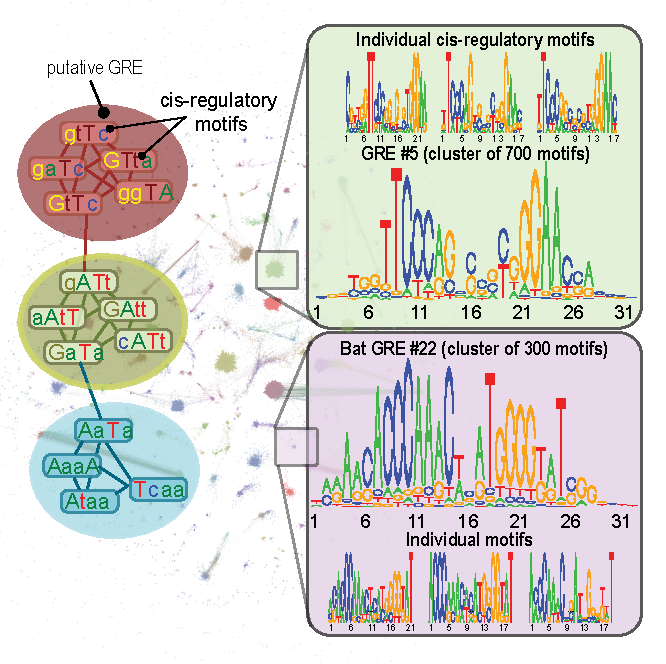
\includegraphics[width=0.6\linewidth]{figures/gre_clustering.pdf}
%\epsfig{file=figures/e2.eps,width=0.8\linewidth}
%\vspace{5in}
\caption[Motif clustering and GRE identification]{
\textbf{Motif clustering and GRE identification.} (Left) A schematic of the approach used to align and cluster individually detected motifs to define GREs. In this example, similar motifs were aligned and clustered into three GREs using Tomtom and mcl (Details in Methods and Supplementary Methods). (Center) The {\it H. salinarum} network of aligned and clustered motifs. (Right) Two {\it H. salinarum} GREs discovered by this method. The motif logo of each GRE was generated by summing PSSMs of the individual aligned motifs in the cluster, as illustrated by three examples of individual motifs (prior to alignment) for each of the two GREs. Note that relative to the individual motifs, the averaged GRE motif is more palindromic - a hallmark of binding sites for dimeric TFs.}
\label{fig:gre_clustering}
%\vspace{-.1in}
\end{figure}

\subsection{Genome-wide scanning of motifs to obtain GRE locations}
\label{section:scanning}

We used motif scanning to discover GRE locations that were missed by the rigid definition of a promoter in \cm\ (typically -250 to +50 nucleotides surrounding the translation start site). This procedure was critical for discovering GREs in non-canonical locations, such as internal to operons. We computed how well each PSSM (described above) matched every position in the genome using \tmsamp{MAST} \cite{bailey_methods_1998}, and recorded significant matches at each genomic location subject to a position $p$-value threshold of $10^{-5}$. This $p$-value cutoff corresponds to an expectation of discovering $\sim 20$ sites at random across the genome. For each GRE, we summed the number of significant matches to each of the GRE’s PSSMs at each genomic position. These counts were used to represent GRE composition in promoters (Figure \ref{fig:egrin2:2:C} and Figure \ref{fig:egrin2:2:D}). In addition, we used these scanned locations to identify GREs located predominantly inside coding regions. Since these GREs may be spurious (\eg, protein sequence motifs or trinucleotide patterns) they were flagged, although they were not removed from our global analysis.

We compared the genome-wide distribution of GRE locations to annotated start sites in \textit{H. salinarum}.  We discovered that most GREs occur in consistent locations with respect to gene start sites.  The global position of all GREs and select GREs relative to experimentally determined gene start sites is depicted in Figure \ref{fig:gre_global_locs_hal}.

\begin{figure}[h!]
\centering
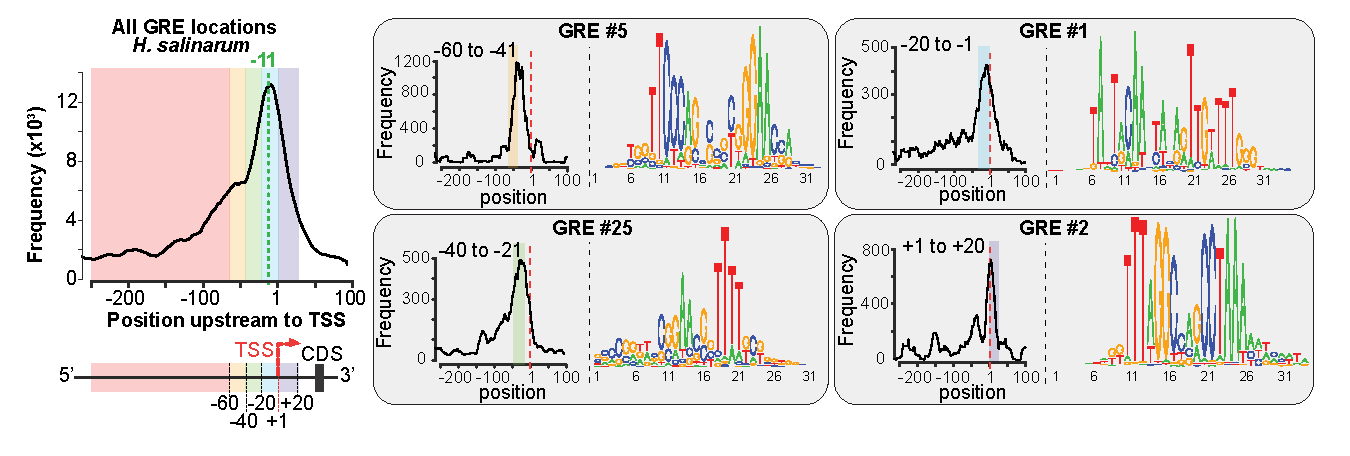
\includegraphics[width=0.95\linewidth]{figures/gre_global_locs_hal.pdf}
\caption[Genome-wide distribution of GREs relative to experimentally mapped transcriptional start sites in \textit{H. salinarum}]{\textbf{Genome-wide distribution of GREs relative to experimentally mapped transcriptional start sites in \textit{H. salinarum}.}  (Left) Predicted positions for all GREs in gene promoters upstream of experimentally mapped transcription start sites (TSSs; \cite{koide_prevalence_2009}) in and (Right) four example elements. Distribution peaks for most GREs occur at characteristic locations. For instance, the location of TATA box-like elements (GRE \#25) between -21 to -40 nt upstream to TSSs in {\it H. salinarum} is consistent with the characterized location of basal elements in archaeal promoters (-25 to 30 nt upstream to TSS). GRE location enables prediction of putative roles for the cognate TF (\eg repressor, activator or a basal factor).} 
\label{fig:gre_global_locs_hal}
\end{figure}

\subsection{Detection of co-regulated modules (corems) by community detection}

\subsubsection{Construction of gene-gene co-occurrence network}
\label{section:gBg}

We post-processed the \egrine~ensemble to refine the underlying network structure and discover functionally meaningful gene co-regulatory modules present in the model. To do so, we transformed the ensemble of biclusters into a weighted gene-gene association graph $G$, where the nodes of $G$ are genes and the weight of edges between the nodes is proportional to their frequency of co-occurrence in biclusters:

\begin{equation}
w_{ij} = \frac{\left|B_i\cap B_j\right|}{\mathrm{min}(B_i,B_j)},
\end{equation}

\noindent where $w_{ij}$ is the weight of the edge between genes $i$ and $j$, $B_i$ is the set of all biclusters containing gene $i$. The weights were normalized by the minimum number of biclusters containing either gene, rather than by the more typically applied union (which would make the score identical to the Jaccard Index) to avoid penalizing genes that occur infrequently in biclusters. The sum of edge weights for each gene was normalized to one. This gene-gene co-occurrence network represents how often \cm~ discovers co-regulation between every pair of genes in the genome. We note that since this network is derived from biclusters, it is also a reflection of conditional co-expression and predicted \textit{cis}-­regulatory motifs.

\subsubsection{Network backbone extraction}

After transforming the ensemble into a normalized graph, we removed edges that were statistically indistinguishable by multiscale backbone extraction (null hypothesis of uniform edge weight distribution given a node of degree $k$) \cite{serrano_extracting_2009}. We retained all edges satisfying the following relation:

\begin{equation}
\alpha_{ij}=1-(k-1)\int_0^{w_{ij}}(1-x)^{k-2}dx\leq 0.05,
\end{equation}

\noindent where $\alpha_{ij}$ is the probability that the normalized weight $w_{ij}$ between genes $i$ and $j$ is compatible with the null hypothesis, and $k$ is the degree of gene $i$. For \halo, backbone extraction reduced the number of regulatory edges from 1,576,643 to 141,667; in \eco~ the number of edges was reduced from 3,094,954 to 170,723.

\subsubsection{Network link-community detection}
\label{section:linkcommunity}
Following backbone extraction, we detected corems by application of a recently described link-community detection algorithm \cite{ahn_link_2010}. For this algorithm to work on our data set we modified it to accept input of a weighted graph \cite{kalinka_linkcomm:_2011}. We implemented it in \tmsamp{C++} for efficiency. The algorithm computes a similarity score between all pairs of edges sharing a common keystone node, $k$, according to the Tanimoto coefficient, $T$:

\begin{equation}
T(e_{ik},e_{kj}) = \frac{a_i\cdot a_j}{|a_i|^2+|a_i|^2+a_i\cdot a_j},
\end{equation}

\noindent where

\begin{equation}
a_i=w_{ij}+\frac{\delta_{ij}}{k_i}\sum_{l\in n(i)}w_{il}.
\end{equation}

\noindent Here, $e_{ik}$ is the edge between gene $i$ and the keystone gene $k$, and $\delta_{ij}$ is the Kroenecker delta. The score reflects the similarity of gene neighborhoods adjacent to two edges sharing a gene, with the score increasing in value as the number and weight of overlapping adjacent edges increases. To transform the Tanimoto coefficient into a distance metric, we compute $1-T$.

Following scoring, the edges were aggregated by standard hierarchical clustering. The resulting tree is cut at many thresholds to optimize the local weighted density $D$ of the resulting clusters:

\begin{equation}
D=\frac{1}{M\langle w\rangle}\sum_{c\in C}m_c\langle w\rangle_c\left(\frac{m_c-(n_c-1)}{n_c(n_c-1)/2-(n_c-1)}\right),
\end{equation}

\noindent where $M$ is the total number of edges in the entire network, $\langle w\rangle$ is the average weight of edges in the entire network, $C$ is the set of all link communities at a given threshold, $m_c$ is the number of edges in community $c$, $\langle w\rangle_c$ is the average weight of edges in community $c$, and $n_c$ is the number of genes in community $c$. The density scoring metric $D$ had a clear optimum corresponding exactly to the cutoff that would have been chosen had we used the unweighted scoring metric originally described (Figure \ref{fig:corem_density}). Only communities with more than two genes were retained.

\begin{figure}[h!]
\centering
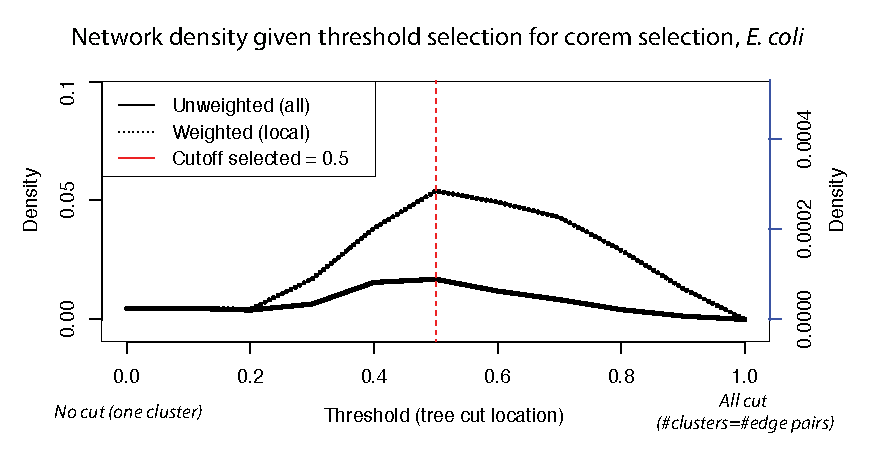
\includegraphics[width=0.9\linewidth]{figures/corem_density.pdf}
\caption[Corem density as a function of clustering cutoff threshold]{{\bf Corem density as a function of clustering cutoff threshold.} Hierarchical clustering cut threshold chosen to maximize the density of resulting clusters. The cutoff chosen with modified weighted density metric is identical to unweighted density metric.} 
\label{fig:corem_density}
\end{figure}

Since the communities produced by this algorithm are comprised of sets of edges, we defined a corem to include all genes incident to the edges in a community. Because of this definition, each gene can be a member of multiple different corems. In {\it H. salinarum}, this procedure generated 679 corems ranging in size from 3 to 377 genes, covering 1,363 of the 2,400 genes in the genome, and comprising 56,738 co-regulatory associations. In {\it E. coli}, we discovered 590 corems, ranging in size from 3 to 153 genes, covering 1,572 of 4,213 genes and 25,976 regulatory edges. See Table\ref{tab:stats} and Figure \ref{fig:corem_density} for additional statistics. Gene-to-corem and corem-to-gene mappings for the {\it H. salinarum} and {\it E. coli} models are available online.

\begin{figure}[h!]
\centering
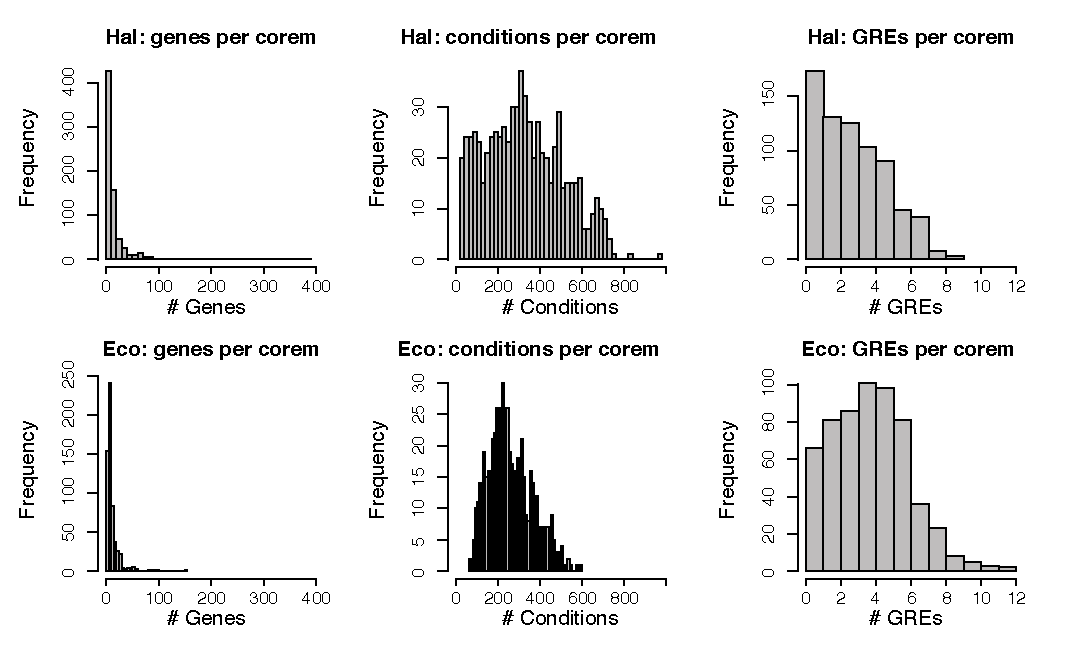
\includegraphics[width=0.9\linewidth]{figures/corem_stats.pdf}
\caption[Corem statistics]{
{\bf Corem statistics.} Number of genes, conditions, and GREs per corem for \textit{E. coli} and \textit{H. salinarum} \egrine~models.} 
\label{fig:corem_stats}
\end{figure}

\section{Model Evaluation}

In this section we evaluate the performance of the \egrine\ model as a function of several important parameters. We focus in particular on how the performance of the model changes as a function of the number of runs included. From these evaluations, we conclude that (1) the model performs well in its final form, (2) the model has reached a stable-state wherein inclusion of additional runs does not significantly increase model performance, and (3) the model is not over-fit to particular experiments within a data set or to any data set as a whole.

\subsection{Comparison with other module detection algorithms}

We compared the number of \rdb~TFs detected in the \egrine~model to individual \cm~runs as well as to several other module detection/clustering algorithms that were computed on subsets of the experimental data (similar to the \egrine~ensemble; Figure \ref{fig:ensemble_comparison_regDB}). We evaluated: (a) $k$-means clustering, (b) \tmsamp{WGCNA} \cite{langfelder_wgcna:_2008}, and (c) \tmsamp{DISTILLER} \cite{lemmens_distiller:_2009}. For (a) and (b), we computed modules 100 times on random subsets of the {\it E. coli} expression data set (using 200-250 randomly chosen experiments per run; selection criteria were identical to {\it E. coli} \egrine). We then predicted {\it de novo cis}-regulatory GREs in the promoter regions of genes in each module using \tmsamp{MEME} (\tmsamp{MEME} parameters were also identical to \egrine). For (c), we performed the comparison using the original modules generated by \cite{lemmens_distiller:_2009}. Rather than alter module composition by re-detection, we instead varied \tmsamp{MEME} parameters applied to the modules 100 times (again, within the same ranges as those used for \egrine). TF-GRE matches were assigned by comparing GREs to \rdb~TF binding sites, as previously described (Section~\ref{section:tfbs:vs:regdb}).

We found that individual \cm~runs discovered a greater number of \rdb~binding sites, on average, than the other methods (an average of 41 for \cm, compared to averages of 30, 25, and 29 for $k$-means, \tmsamp{WGCNA}, and \tmsamp{DISTILLER}, respectively), which is consistent with previous findings \cite{reiss_integrated_2006} (Figure~\ref{fig:ensemble_comparison_regDB}). Integration of all \cm~biclusters into the complete \egrine~ensemble outperformed all individual \cm~runs (53 total, as described in the Manuscript). This result is typical of ensemble-based inference approaches, and supports the value of ensemble integration as part of the \egrine\ model.

\begin{figure}[h!]
\centering
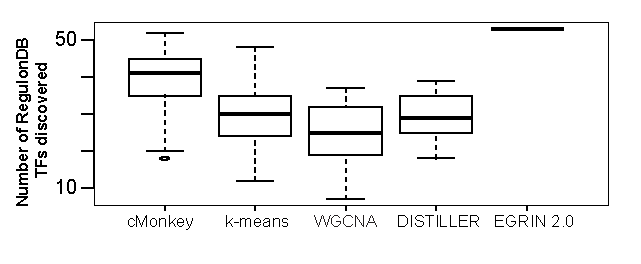
\includegraphics[width=0.6\linewidth]{figures/ensemble_comparison_regDB.pdf}
\caption[Number of TFs in \rdb~ re-discovered by various regulatory module detection methods.]  {{\bf Number of TFs in \rdb~ re-discovered by various regulatory module detection methods.} Comparison of \egrine~ (solid line, far right) to individual \cm\ runs, as well as multiple runs of $k$-means, \tmsamp{WGCNA}, and \tmsamp{DISTILLER} on subsets of the expression data. Evaluation made with respect to re-discovery of binding sites for 88 TFs with $\geq 3$ unique sites in \rdb~ based on genome-wide binding site locations (FDR $\leq 0.05$).} 
\label{fig:ensemble_comparison_regDB}
\end{figure}

\subsection{Convergence and stability of inferred GRNs}

To evaluate the stability of the inferred \egrine\ network, we quantified how the model changes as individual \cm\ runs are excluded from the ensemble. Since the sub-bagging, as performed for the \egrine\ model inference, reduce model over-fitting, we used this evaluation understand whether the model is over-fit to particular experiments in the data set. For this task, we computed the number of individual EGRIN runs required to converge on a consistent gene-gene co-occurrence network (see Section \ref{section:gBg}). We computed gene-gene co-occurrence networks based upon randomly selected subsets of the 106 available \eco\ \cm\ runs, and varied the percentage selected between 1\%-99\% of the 106 runs. 5 replicate samples were computed for each. To compare the networks, we computed the Pearson correlation between the two matrices (sub-sampled gene-gene co-occurrence versus the final \egrine\ gene-gene co-occurrence network). Note that since the gene-gene co-occurrence network is a weighted adjacency matrix, the correlation reflects the weighted discovery rate for every pair of genes (rather than simple presence/absence). In Figure \ref{fig:gBg_network_converge} we demonstrate that the underlying networks converge rapidly to the final solution. By the time $\sim 50$\% of the runs have been included ($\sim 50$ runs), the inferred network is nearly identical to the final network ($\sim 100$ runs; cor $> 0.9$). The backbone extracted network takes a slightly longer time to converge, likely because it requires more observations of gene-gene pairs to retain them in the final network. Since corem detection is deterministic and strictly based on the underlying gene-gene co-occurrence matrix, this convergence means that the inferred corems would be nearly identical even if up to half of the runs were excluded.

\begin{figure}[h!]
\centering
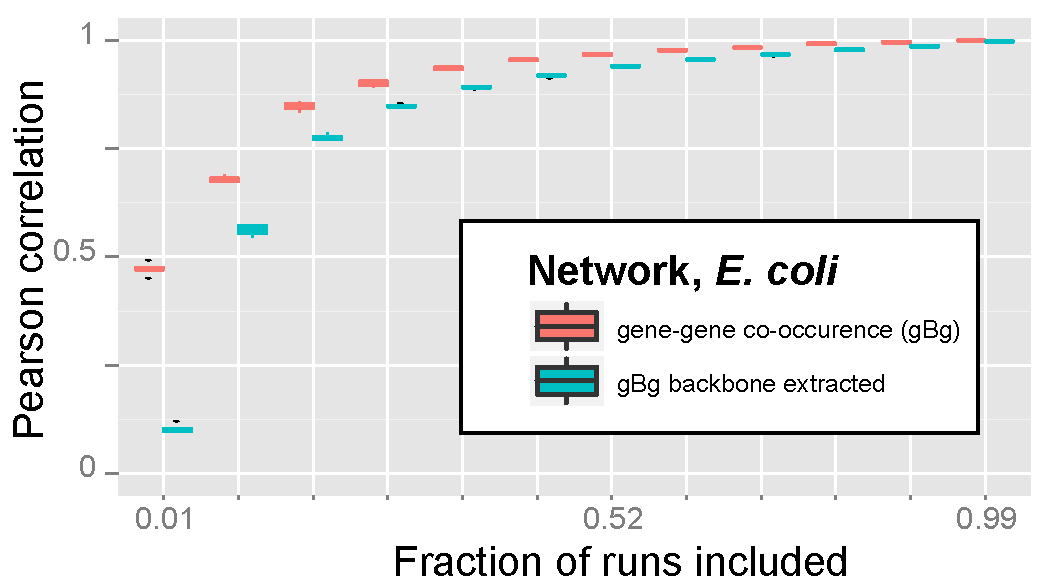
\includegraphics[width=0.75\linewidth]{figures/gBg_network_converge.pdf}
\caption[Convergence of \egrine\ gene co-occurrence networks.]  {{\bf Convergence of \egrine\ co-occurrence networks.} The co-regulation of genes predicted by the \eco\ \egrine\ model converges rapidly to a stable network. Shown is the similarity of the gene-gene co-occurrence matrix (and the backbone extraction of this matrix) to the final \egrine\ \eco\ network, computed when varying fractions of the \cm\ runs were excluded (Pearson correlation vs. the complete model). Each point contains a box plot representing 5 replicate sub-samples.} 
\label{fig:gBg_network_converge}
\end{figure}

\subsection{Confirmation of corems in an independent data set}

To determine whether \egrine\ model predictions are over-fit to the \tmsamp{DISTILLER} expression compendium (or are the result of biases in that data set), we tested whether support for corems existed in an independent {\it E. coli} expression data set. Such evidence would suggest that corems are \textit{bona fide} gene regulatory modules that can be re-discovered in independent data, and that their degree of condition-specificity is not biased due to normalization differences in any given data set. For this test, we used the \tmsamp{DREAM5} gene expression compendium. As described above (Section \ref{section:dream5_data_compendium}), this data set is comprised of different conditions, array platforms, and, most important, was normalized by different methods, than the \tmsamp{DISTILLER} data set used for model training. We determined the condition-specific activity of corems in the \tmsamp{DREAM5} data set using the methods described in Section \ref{section:rsd}. If a corem was significantly co-expressed ($p$-value $\leq$ 0.05) in at least one condition, we classified it `supported'. To our surprise, we not only discovered support for $\sim 99$\% of the predicted corems, we also discovered that their conditionality was very similar across both data sets -- \ie, corems discovered to be co-expressed in few conditions in the \tmsamp{DISTILLER} data set are also co-expressed in few conditions in the \tmsamp{DREAM5} data set (same for corems regulated in many conditions), and similarly for corems co-expressed in a large number of conditions (Figure~\ref{fig:corem_conds_distiller_dream5}). Even after we removed the intrinsic relationship between the number of genes in a corem and the number of conditions in which it is co-expressed, we still observed a significant partial correlation of 0.49 ($p$-value $< 10^{-6}$) between the number of conditions in corems as defined from the two data sets.

\begin{figure}[h!]
\centering
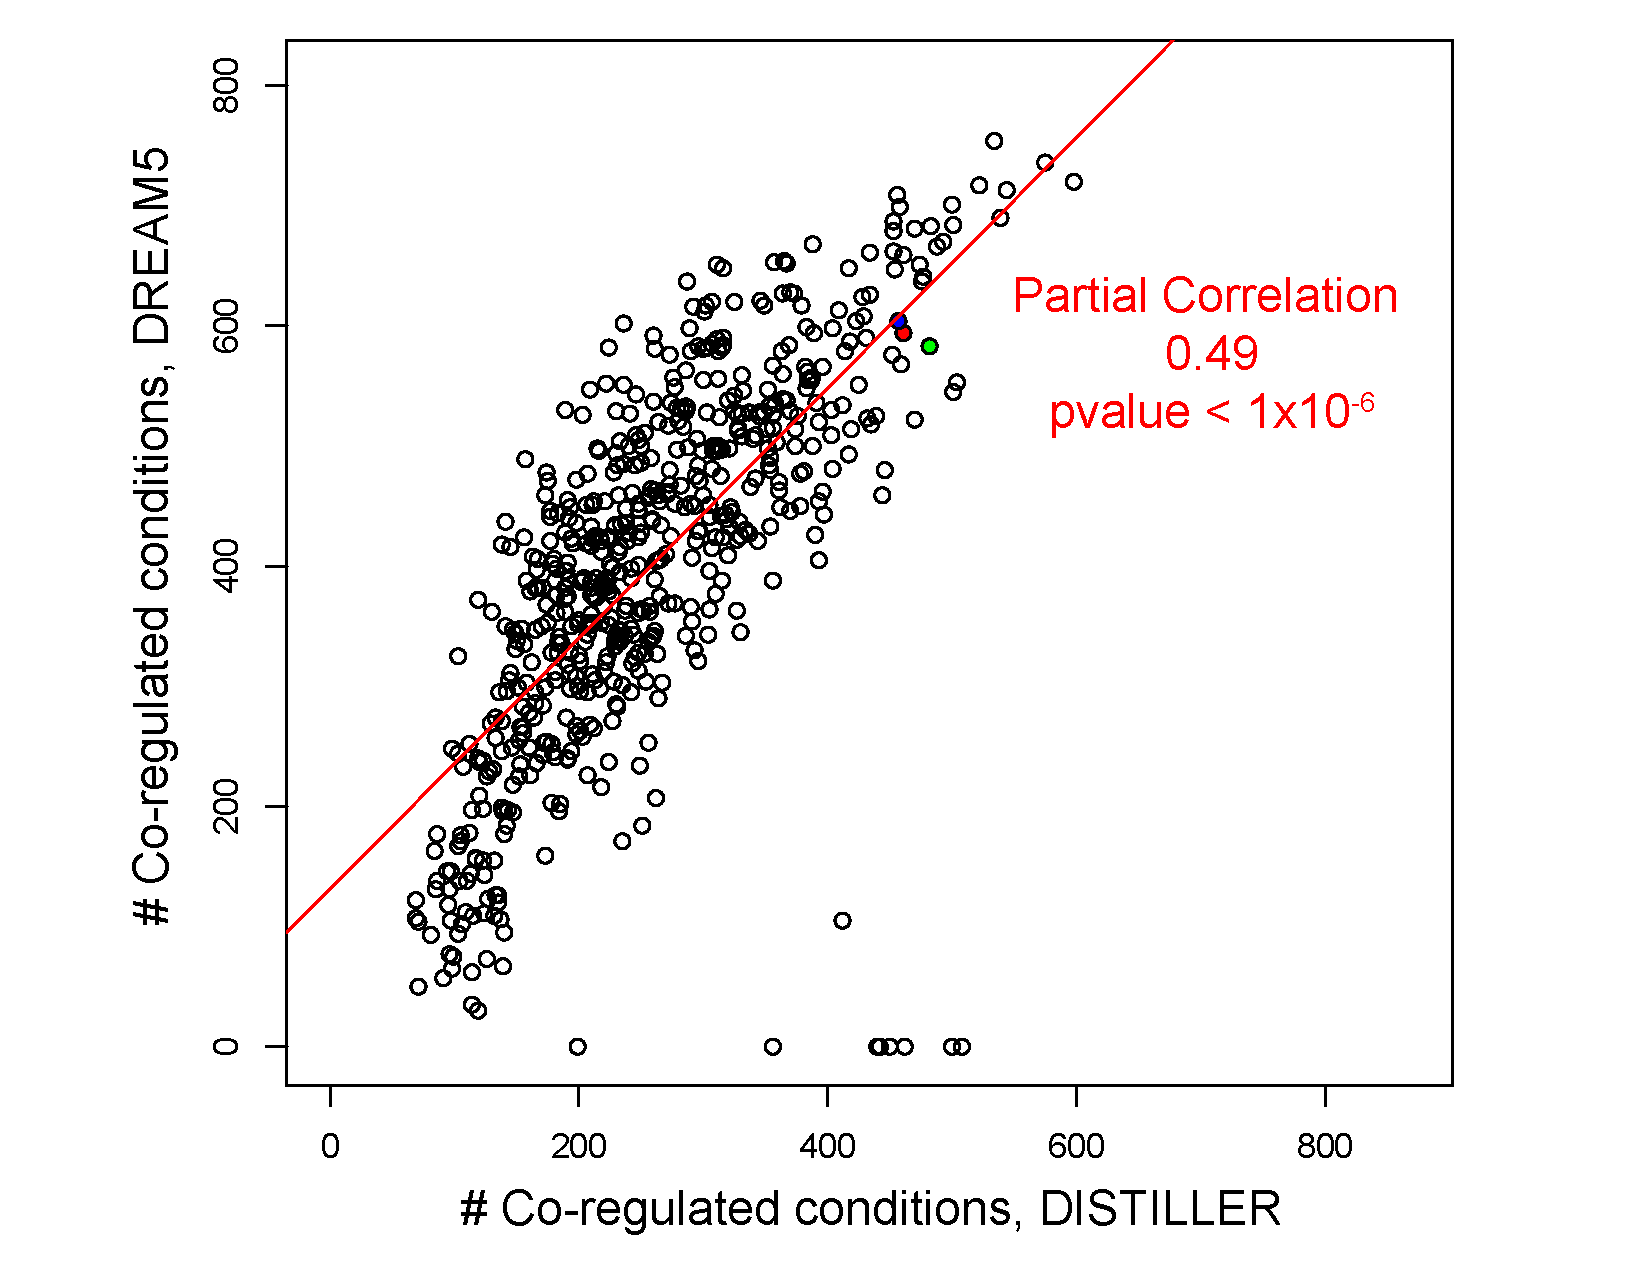
\includegraphics[width=0.6\linewidth]{figures/corem_conds_distiller_dream5.pdf}
\caption[Reproducibility of corems across data sets]{\textbf{Reproducibility of corems across data sets.} Number of co-expressed conditions for corems in the \tmsamp{DISTILLER} and \tmsamp{DREAM5} expression compendia. Conditions were selected as in Section~\ref{section:rsd}. Significant partial correlation of 0.49 is observed after removing the affect of gene set size (log) on the number of conditions co-expressed ($p$-value $< 10^{-6}$). The three corems detailed in the main manuscript are identified with their respective colors ({\color{red}ec512157}, {\color{blue}ec516034}, {\color{green}ec516031})} 
\label{fig:corem_conds_distiller_dream5}
\end{figure}

\section{Model Validation}

\subsection{Data For Model Validation}

\subsubsection{ \halo} \label{halodata}

\paragraph{Tiling array transcriptome measurements}

We generated {\it H. salinarum NRC-1} high-resolution (12 nt) tiling array transcriptome measurements over 12 points along the growth curve in rich media. These were analyzed and published in a separate study \cite{koide_prevalence_2009}. Locations of putative transcription breaks in these data were identified in using multivariate recursive partitioning, including signals from both relative changes in expression along the growth curve, as well as raw RNA hybridization signal.

\paragraph{ChIP-chip transcription factor binding measurements for global regulators}

Global binding of eight general transcription factors (seven TFBs [TFBa, TFBb, TFBc, TFBd, TFBe, TFBf, and TFBg] and one TBP [TbpB]) and three specific TFs (Trh3, Trh4, and VNG1451C) in {\it H. salinarum} were collected in our lab by ChIP-chip. A detailed protocol is described in \cite{facciotti_general_2007}. Briefly, ChIP-enriched and amplified DNA for eleven regulators was hybridized to a low-resolution (500~nt resolution) custom PCR-product array spotted in-house. The resulting intensities were analyzed using {\tmsamp{MeDiChI}} \cite{reiss_model-based_2008} to obtain binding site locations with an average precision of 50~nt. Local false discovery rates (LFDRs) were quantified by simulation.

\paragraph{\textit{kdp} promoter serial truncation measurements}

{\it H. salinarum NRC-1} \textit{kdpFABC} truncation data were obtained from \cite{kixmller_archaeal_2011}. Briefly, the authors measured relative induction of a transcriptional reporter after serial truncation of the \textit{H. salinarum} R1 \textit{kdpFABC} promoter. The authors measured $\beta$-Galactosidase activities from truncated transcriptional fusions of the \textit{kdpFABC} promoter to \textit{bgaH}. $\beta$-Galactosidase activities were measured in triplicate from cultures grown in inducing (3 mM K$^{+}$) and non-inducing (100 mM K$^{+}$) conditions. We obtained data corresponding to Figure \ref{fig:egrin2:2:C}, in which the authors quantify the fractional $\beta$-Galactosidase activity (non-induced/induced) among the serial truncations (private communication). We overlaid motif predictions from \egrine~on this data set to reach our conclusions.

\subsubsection{\eco} \label{ecodata}

\paragraph{Tiling array transcriptome measurements}
\label{section:ecoarray}

We measured \eco\ tiling array transcriptome profiles at nine different time points during growth in rich media (LB). Growth phases spanned lag-phase (OD600 = 0.05) to late stationary-phase (OD600 = 7.3). RNA samples were prepared by hot phenol-chloroform extraction \cite{khodursky_escherichia_2003}. RNA was directly labeled and hybridized to custom Agilent tiling arrays containing 60mer probes tiled across both strands of the \eco\ genome using a sliding window of 23~nt (GEO Platform GPL18392), as in \cite{koide_prevalence_2009}. Expression measurements were quantile-normalized as in \cite{yoon_parallel_2011} and analyzed for condition-specific transcriptional isoforms following the segmentation protocol described in \cite{koide_prevalence_2009}. Data is available on GEO (GSE55879).

\paragraph{PurR/$\Delta$PurR expression data and ChIP-chip transcription factor binding sites} 

{\it E. coli} PurR/$\Delta$PurR expression data and ChIP-chip transcription factor binding measurements collected in the presence of adenine were taken from \cite{cho_purr_2011}. ChIP-chip relative intensities were re-analyzed using {\tmsamp{MeDiChI}} \cite{reiss_model-based_2008} to obtain binding site locations with an average precision of $\sim$25~nt.

\paragraph{Fitness measurements}
\label{section:fitness}

{\it E. coli} fitness measurements across 324 conditions were generated by \cite{nichols_phenotypic_2011}. In short, the authors quantitated growth rates for 3979 single gene deletions in each of 324 environments with variable stress, drug, and environmental challenges. \textit{E. coli} mutant colony sizes were quantified on agar plates.  Fitness correlations were obtained directly from the authors: \href{http://ecoliwiki.net/tools/chemgen/}{http://ecoliwiki.net/tools/chemgen/}. Each correlation value represents the Pearson correlation of fitness (\ie, relative growth rate) for pairs of single gene deletion mutants measured across all 324 conditions that are also present in our analysis. Relative fitness scores were also obtained directly from the authors.

\paragraph{Effector molecule measurements}

{\it E. coli} effector molecule measurements were taken from \cite{ishii_multiple_2007}. The authors measured metabolite levels using capillary electrophoresis time-of-flight mass spectrometry (CE-TOFMS) in \eco, as well as several other biomolecules (\eg., RNA and protein). \textit{E. coli} was grown in a chemostat at several different dilution rates (0.1, 0.2, 0.4, 0.5, and 0.7 hours$^{–1}$). We obtained the metabolite levels from the authors and computed Pearson correlation between metabolites assigned to regulate TFs by RegPrecise \cite{novichkov_regpredict:_2010}.

\paragraph{Experimentally mapped {\it E. coli} transcription factor binding sites}

We compared genome-wide locations of GREs in the {\it E. coli} EGRIN 2.0 model with experimentally-mapped binding sites from the \rdb database \cite{gama-castro_regulondb_2011}. To maintain consistency with our comparisons against the DREAM5 community networks \cite{marbach_wisdom_2012}, we used version 6.8 of the database. For binding sites, we used the {\tmsamp{BindingSiteSet}} table, filtered for only interactions with experimental evidence, and used only TFs with $\geq 3$ unique binding sites -- a total of 88 TFs.

\paragraph{Experimentally measured {\it E. coli} transcription factor regulatory targets}
\label{section:eco:gold:standard}

For the {\it E. coli} gold standard network, we used the same network as that used by \cite{marbach_wisdom_2012} for validation of the DREAM5 {\it E. coli} community predicted regulatory networks. This gold standard is based upon version 6.8 of the \rdb~ database \cite{gama-castro_regulondb_2011}, and only interactions with at least one strong evidence were included, for a total of 2,066 interactions. We mapped the $aaaX$-style gene names in the DREAM5 gold standard to the $b1234$ in \cm~using a translation table compiled in the {\tmsamp{EcoGene}} database, version 3.0 \cite{zhou_ecogene_2013}. We were able to map a total of 4,273 gene names. The final gold standard consisted of 2,064 interactions between 141 TFs and 997 target genes. The final, complete gold standard network used for all analyses is available \href{http://egrin2.systemsbiology.net/}{online}.

\subsection{Computational Methods for Model Validation}

\subsubsection{Functional enrichment estimates for genes in corems}

We computed functional enrichment for genes organized into corems using \tmsamp{DAVID} \cite{dennis_david:_2003} and the \tmsamp{DAVIDQuery} \cite{day_davidquery:_2010} \tmsamp{R}-package. Enrichments for each corem are available on the \href{http://egrin2.systemsbiology.net}{web site}.

\subsubsection{Conditional co-regulation of genes organized in corems}
\label{section:rsd}

We defined the conditions in which genes in a corem were co-regulated as the set of experiments in which the genes of a corem are more tightly co-expressed than one would expect at chance. We statistically evaluated tight co-expression using relative standard deviation (RSD $=|\sigma/\mu|$) by resampling. We chose RSD (rather than, for example, standard deviation, $\sigma$) to avoid over-weighting conditions in which the mean relative expression is close to zero. The significance of an RSD value for a given condition relative to each corem was estimated by resampling: for a corem with $k$ gene members, and for each condition, $c$, we computed at least 20,000 RSD values for $k$ randomly sampled expression measurements in $c$, to determine the likelihood that the observed co-expression has lower RSD than expected by chance ($p$-value $< 0.01$). The resampling procedure resulted in condition sets for corems that contained from 1.4\% to 85.5\% of the conditions in \halo\ and 7.9\% to 66.6\% conditions in \eco\ (Figure \ref{fig:corem_stats}).

\subsubsection{Conditionality of GRE influence}

The upstream promoter regions of most genes contain multiple \egrine-predicted GREs (\eg, \textit{carA} in Figure \ref{fig:egrin2:2:D}). A key insight of our model is that not all of these sites are equally important for controlling gene expression in all experimental conditions. We refer to changes in the relative influence of GREs across conditions as ``conditional activity'' of GRE elements. Although, to be clear, we do not imply that the transcriptional activity at a GRE is attributable to the DNA sequence itself, but rather the TF that binds to that sequence in particular environments. We leveraged the GREs discovered in genes grouped into corems and the conditional co-expression of those groups of genes to predict conditionally active GREs in \egrine.

To identify the active GREs for each corem we combined predictions from (1) genome-wide motif scans (Section~\ref{section:scanning} above) that predict the GRE locations in an expanded region around each gene’s promoter in the corem using all of the ensemble predictions (1,000 nt window: -875 nt upstream to 125 nt downstream), and (2) the conditions discovered in biclusters that are most representative of the corem (\ie, containing the largest fraction of genes from the corem, top decile). GREs that occurred frequently in these biclusters were considered putatively responsible for co-regulating the set of genes in the condition-specific context of the corem ($q$-value $\leq$ 0.05). Finally, we computed the average distances of all GREs to the start codons of each gene in the list (collapsing sites if they occurred within 25 nt of one another). The precise locations of all GREs for the {\it H. salinarum} \textit{dpp} operon-related corems (Figure \ref{fig:egrin2:3:A}) are available in Table S8 of the corresponding paper, while the locations of GREs involved in conditional modulation of the PurR regulon (\ref{fig:egrin2:4:A}) are provided in Table S9.

We represented the active GREs upstream of a gene or within a corem as a pie chart, showing the normalized frequency with which the GREs computed above occurred in biclusters containing that gene. For example, if GREs 1, 2, and 3 occurred in 25, 50, and 200 biclusters containing gene $A$, the pie chart for gene $A$ would have sectors of area 0.09, 0.18, and 0.73 respectively. For corems, we computed the normalized frequency of GREs for all genes of the corem. For example, if GREs 1, 2, and 3 occurred in promoters of 10, 10, and 20 of the genes of the corem, their areas would be 0.25, 0.25, and 0.5 respectively.

\begin{figure}[h!]
\centering
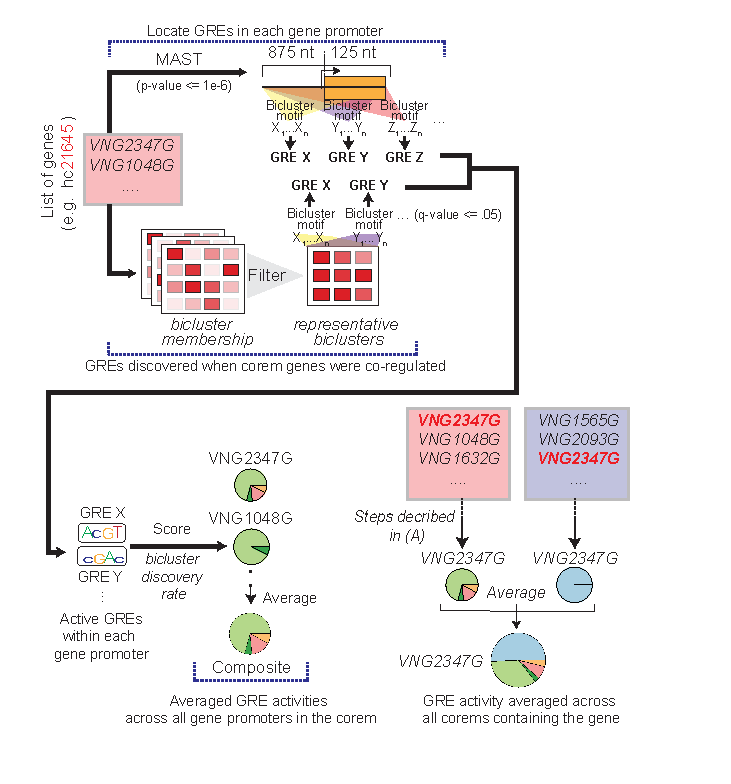
\includegraphics[width=0.7\linewidth]{figures/corem_gres.pdf}
\caption[Deciphering GREs responsible for regulating corems]{\textbf{Deciphering GREs responsible for regulating corems.} A GRE is implicated in regulation of a corem when it is both (1) located within an expanded region (-875nt to +125nt) around the translation start site of any gene in the corem; and (2) present in biclusters containing a large fraction of corem genes (top decile). Relative GRE influence is computed as the frequency with which each GRE was discovered in these representative biclusters (see Supplementary Methods for more details). Influence scores are illustrated as pie charts and reported for each gene individually (\eg, \textit{VNG2347G}); and as a composite by averaging across all genes in a corem. The width of each sector in the pie charts is proportional to the frequency of GRE discovery.}
\label{fig:corem_gres}
\end{figure}

\subsubsection{Detection of conditional operons}
\label{section:condop}
Condition-specific transcriptional isoforms of operons were predicted through corem membership. If any of the genes in an operon were found in a corem that did not contain all the other genes of the operon, we predicted that the operon had conditional isoforms. Operon annotations for both {\it H. salinarum} and {\it E. coli} were derived from \tmsamp{MicrobesOnline} \cite{alm_microbesonline_2005}. All predicted conditional operons, including the specific break sites and transcriptional isoforms is available on the website. The full list of validated predictions is provided in Table S7.
\subsubsection{Environmental ontology construction and usage}

We recorded a rich set of meta-data for all 1,495 experiments conducted with {\it H. salinarum} and used for construction of the \halo~ \egrine~model. The meta-data includes a detailed description of each experiment, including, for example: media composition, genetic background, concentration of perturbant, internal reference batch id, person who conducted the experiment, etc. We used this meta-information to classify experiments in an ontological framework, where two experiments can share specific meta-descriptions (\eg, $10^{-3}$ mol/L EDTA), or inherit more general relationships from the ontological structure (\eg, chemical perturbation). We used OBO-edit \cite{day-richter_obo-editontology_2007} to construct the ontology. The ontology contained 198 terms organized across three primary branches (environmental state, experimental state, and genetic state). The ontology flat file is available for download and meta-data annotations for every array in the dataset are available \href{http://egrin2.systemsbiology.net}{online}.

\begin{figure}[h!]
\centering
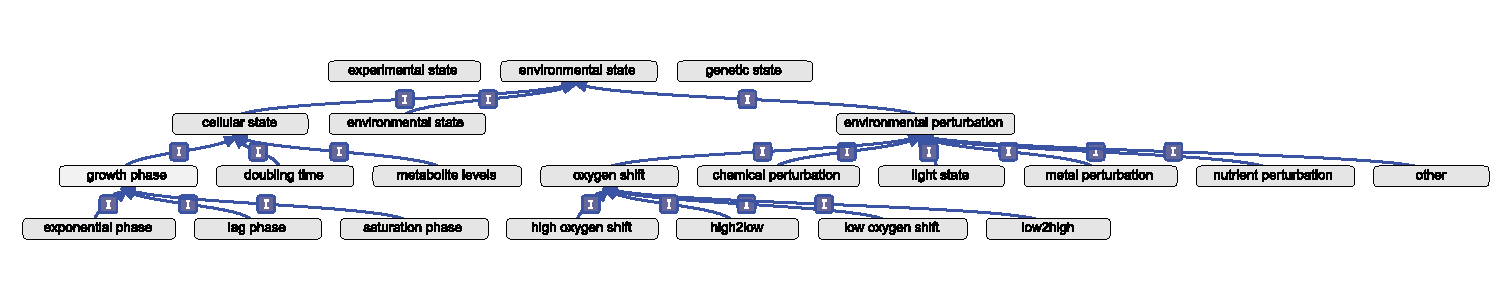
\includegraphics[width=0.95\linewidth]{figures/eo.pdf}
\caption[Environmental ontology hierarchically organizes relationships between experimental conditions from metadata collected across 1495 experiments in \textit{H. salinarum}]{{\bf Environmental ontology hierarchically organizes relationships between experimental conditions from metadata collected across 1495 experiments in \textit{H. salinarum}.} Subset of the environmental ontology constructed for \textit{H. salinarum} demonstrates many “is-a” (boxed ‘I’) relationships that organize similarities between descriptor terms descending from one of three root nodes (i.e., generic categorical descriptions). In this case a generic ontological term called `environmental state' gives rise to much more specific terms (e.g., exponential phase or high oxygen shift) that inherit (at the highest level) a relationship through their being related to the ‘environmental state’ of cells in the experiment. Each condition in the compendium is annotated with the most specific descriptors relevant to the experiment given metadata. The full environmental ontology is available for download from \href{http://egrin2.systemsbiology.net}{http://egrin2.systemsbiology.net}.}
\label{fig:eo}
\end{figure}

We used the ontology to classify enriched environmental features for GREs and corems. For corems, we used the set of conditions in which genes in the corem are significantly co-expressed (see Section \ref{section:rsd} above) to compute term enrichment using the \tmsamp{ontoCAT} \cite{kurbatova_ontocat:_2011}  \tmsamp{R}-package. Term enrichment was assessed statistically and reported as $q$-values using the hypergeometric test with Benjamini-Hochberg correction for multiple hypothesis testing.


\subsection{Global validation of GREs predicted by \egrine}
\label{section:tfbs:vs:regdb}

We compared the genome-wide locations of predicted GREs in the {\it E. coli} \egrine~model to experimentally mapped TF binding sites from \rdb~(BindingSiteSet table, filtered for experimental evidence and TFs with $\geq 3$ unique binding sites; a total of 88 TFs). We considered a GRE to be a significant match to a TF if a significant fraction ($q$-value $\leq 0.05$) of its predicted non-coding locations overlapped with the known binding locations for a particular TF (hypergeometric $p$-value $\leq 0.01$; see GRE definition in Section~\ref{section:gres}). In cases where a GRE significantly matched multiple TFs, only the most significant was reported.

We observed several instances where more than one GRE significantly matched the same TF. We were unable to determine whether this was the result of incomplete GRE clustering, ambiguities related to GRE scanning, limitations of the experimental data itself, or a reflection of subtle context-dependent variations in the binding preferences of these TFs. Since we did not observe clustering of GREs that map to the same TF upon re-clustering, we hypothesize that the observations may have biological origins, \ie, reflect condition-dependent variations in TF binding preferences that are the result, for example, of co-activator/repressor interaction or small molecule binding. It is interesting to note that TFs with the largest fraction of GRE matches include transcriptional dual regulators, such as FlhDC and UlaR (\ie, TFs with the ability to act as both activators and repressors). This is consistent with the observation that these TFs have context-dependent binding preferences. The complete set of validations, for both TFs and $\sigma$-factors, is listed in Table~S4.

\subsection{Global validation of regulatory interactions predicted by \egrine}
\label{section:aupr:vs:regdb}

We assessed the ability of the \egrine\ model to correctly infer known regulatory interactions using the \rdb\ database as a standard metric for comparison. Comparison to the \rdb\ gold-standard is common practice for evaluating model performance \cite{marbach_wisdom_2012}. We performed our evaluation with the version of \rdb~ used by the DREAM5 ensemble (based on \rdb\ release 6.8 \cite{marbach_wisdom_2012}) so that we could directly compare our results. The authors \cite{marbach_wisdom_2012} restricted the gold-standard to well-established interactions, annotated in \rdb\ with the `strong evidence' classification. In all cases, networks were integrated from predictions among the ensemble using an approach similar to that of \cite{marbach_wisdom_2012}, with subtle variations noted in each section, below. To facilitate a direct comparison, we reconstructed a new {\it E. coli} \egrine\ model using the same DREAM5 expression consortium as was used for the original DREAM5 competition (Section~\ref{section:dream5_data_compendium}). The predictions of this model were used {\it solely} for global validation and direct comparison with the DREAM5 community network, as described in this subsection.

We performed two global evaluations of the {\it E. coli} \egrine: (1) a comparison of the GREs detected in the model with experimentally mapped TF binding sites in \rdb~(Section~\ref{section:tfbs:vs:regdb}), and (2) a comparison of the predicted (TF $\rightarrow$ gene) regulation in \egrine~with the gene regulatory network from \cite{marbach_wisdom_2012}. For (2), we computed predicted regulatory networks from \egrine~in two ways: (a) direct (TF $\rightarrow$ target) predictions from \nwinf~ (Section~\ref{sec:nwinf_network}, and (b) a gene regulatory network derived from predicted GREs that were matched to TFs in \rdb~(Section~\ref{section:gre_grn_construction}). Construction of each of these networks is described in detail below (Section~\ref{sec:nwinf_network} and Section~\ref{section:gre_grn_construction}). The methods for, and results of the comparisons are described in Section~\ref{sec:network_comparisons}.

\subsubsection{Conversion of \egrine~\nwinf~influence predictions into a GRN}
\label{sec:nwinf_network}

We computed a direct (TF $\rightarrow$ gene) inferred {\it E. coli} gene regulatory network (GRN) from the \nwinf~predictions in the \egrine~ensemble. As with the original EGRIN model \cite{bonneau_predictive_2007}, \nwinf~influence predictions were originally made between the 296 putative {\it E. coli} TFs (Section \ref{section:eco_tfs}) and each of the $\sim 40,000$ biclusters in the ensemble. We then used a weighted average of the predicted influences among all networks in the ensemble, as follows. If \nwinf~predicted a (TF $\rightarrow$ bicluster) influence with weight $\beta$ then we added $\beta$ to a regulatory interaction between that TF and all genes in that bicluster. Weights $\beta$ were summed for each recurrence of the same (TF $\rightarrow$ gene) interaction. Note, we did not use $|\beta|$ in the individual sums, since we considered contradicting evidence to be cancelling rather than reinforcing. Finally, all (TF $\rightarrow$ gene) interactions in the final network were ranked by absolute total weight (here we {\it did} use $|\beta|$). As with the DREAM5 competition networks, the top 100,000 rankings were retained in the final network. The final \egrine~\nwinf~influence network is available \href{http://egrin2.systemsbiology.net/}{online}. 

\subsubsection{Conversion of \egrine~GRE detections into a predicted GRN}
\label{section:gre_grn_construction}

We computed a separate inferred {\it E. coli} gene regulatory network from predicted GREs in \egrine\ that were matched to TFs as described in Section~\ref{section:tfbs:vs:regdb}. We would like to stress that this inference relies upon (in this case, for {\it E. coli}) annotated binding sites for regulators, which could be statistically linked to predicted GREs through significant overlaps in their genomic locations. This enables inference of (TF $\rightarrow$ gene) direct influence predictions through the indirect relationship:

\begin{equation}
\label{eq:gre_network_relation}
\mathrm{TF} \overset{\mathrm{anno.}}{\rightarrow} \mathrm{GRE} \overset{\mathrm{pred.}}{\rightarrow} \mathrm{gene}.
\end{equation}

\noindent Thus for an understudied organism, such as {\it H. salinarum}, such a network of (TF $\rightarrow$ gene) influences could {\it not} be inferred; rather a (GRE $\rightarrow$ gene) interaction network would be the final product. Such a network still contains predictions which could be validated and acted upon, for example, for engineering purposes. A future direction of our research will be to statistically link TFs to predicted GREs, for example using direct GRN predictions such as those described above (\eg\ Section~\ref{sec:nwinf_network}, or \cite{marbach_wisdom_2012}).

(GRE $\rightarrow$ gene) predictions (in Eq.~\ref{eq:gre_network_relation}) were extracted from the \egrine\ model directly using the \MEME\ predictions for motif instances in the promoters of genes in each of the $\sim$40,000 \cm\ biclusters. We then used an unweighted average of the predictions among all bicluster in the ensemble, as follows. A (TF $\rightarrow$ gene) edge with a weight of 1 was added to the predicted network if the annotated binding sites for that TF could be matched with locations of a motif (Section \ref{section:tfbs:vs:regdb}), which was detected by \MEME\ in a bicluster in the promoter of the gene. Edge weights (1) were added for each additional prediction, in the ensemble of biclusters, of the same (TF $\rightarrow$ gene) interaction. As with the \nwinf~influence network (Section \ref{sec:nwinf_network}), the top 100,000 rankings were retained in the final network. The final \egrine~GRE-based network is available \href{http://egrin2.systemsbiology.net/}{online}. 

\subsubsection{Integration of predicted \egrine~\nwinf- and GRE-based GRNs}

Prior to integration of the two different predicted GRNs described above (Sections~\ref{sec:nwinf_network} and~\ref{section:gre_grn_construction}), we ensured that they were both equally represented in the integrated GRN by re-scaling their weights so that their sums would be equal. The GRNs were then combined into a single, integrated predicted \egrine\ GRN by simply summing the re-scaled weights for any edge predicted in both networks. Thus, this final network integration was a form of weighted average of the two (GRE and \nwinf) networks. This is {\it not} identical to the weighted rank average method described by \cite{marbach_wisdom_2012}, as it does not use a posteriori assessments of each network to assign their relative weights; rather the weights are simply adjust so that each network contributes equally to the predictions.

\subsubsection{Network comparisons and global performance assessments}
\label{sec:network_comparisons}

To compare \egrine\ performance to the DREAM5 ensemble, we computed standard precision-recall statistics for each network using the previously described DREAM5 gold standard GRN.  We computed area-under-the-precision-recall (AUPR) statistics to summarize the predictive performance. AUPR statistics were compared directly with the DREAM5 community ensemble network. By extension, the \egrine~AUPR performance can be compared to the individual best performers in DREAM5 as well (Figure~\ref{fig:egrin2:2:A} in \cite{marbach_wisdom_2012}). The results of these analyses are summarized in Figure~\ref{fig:egrin2:2:A} in the main text. We have made all network predictions available \href{http://egrin2.systemsbiology.net/}{online}. Complete precision-recall curves are shown in Figure~\ref{fig:pr_curves}. The curves are also available in tabular form \href{http://egrin2.systemsbiology.net/}{online}.

\begin{figure}[h!]
\centering
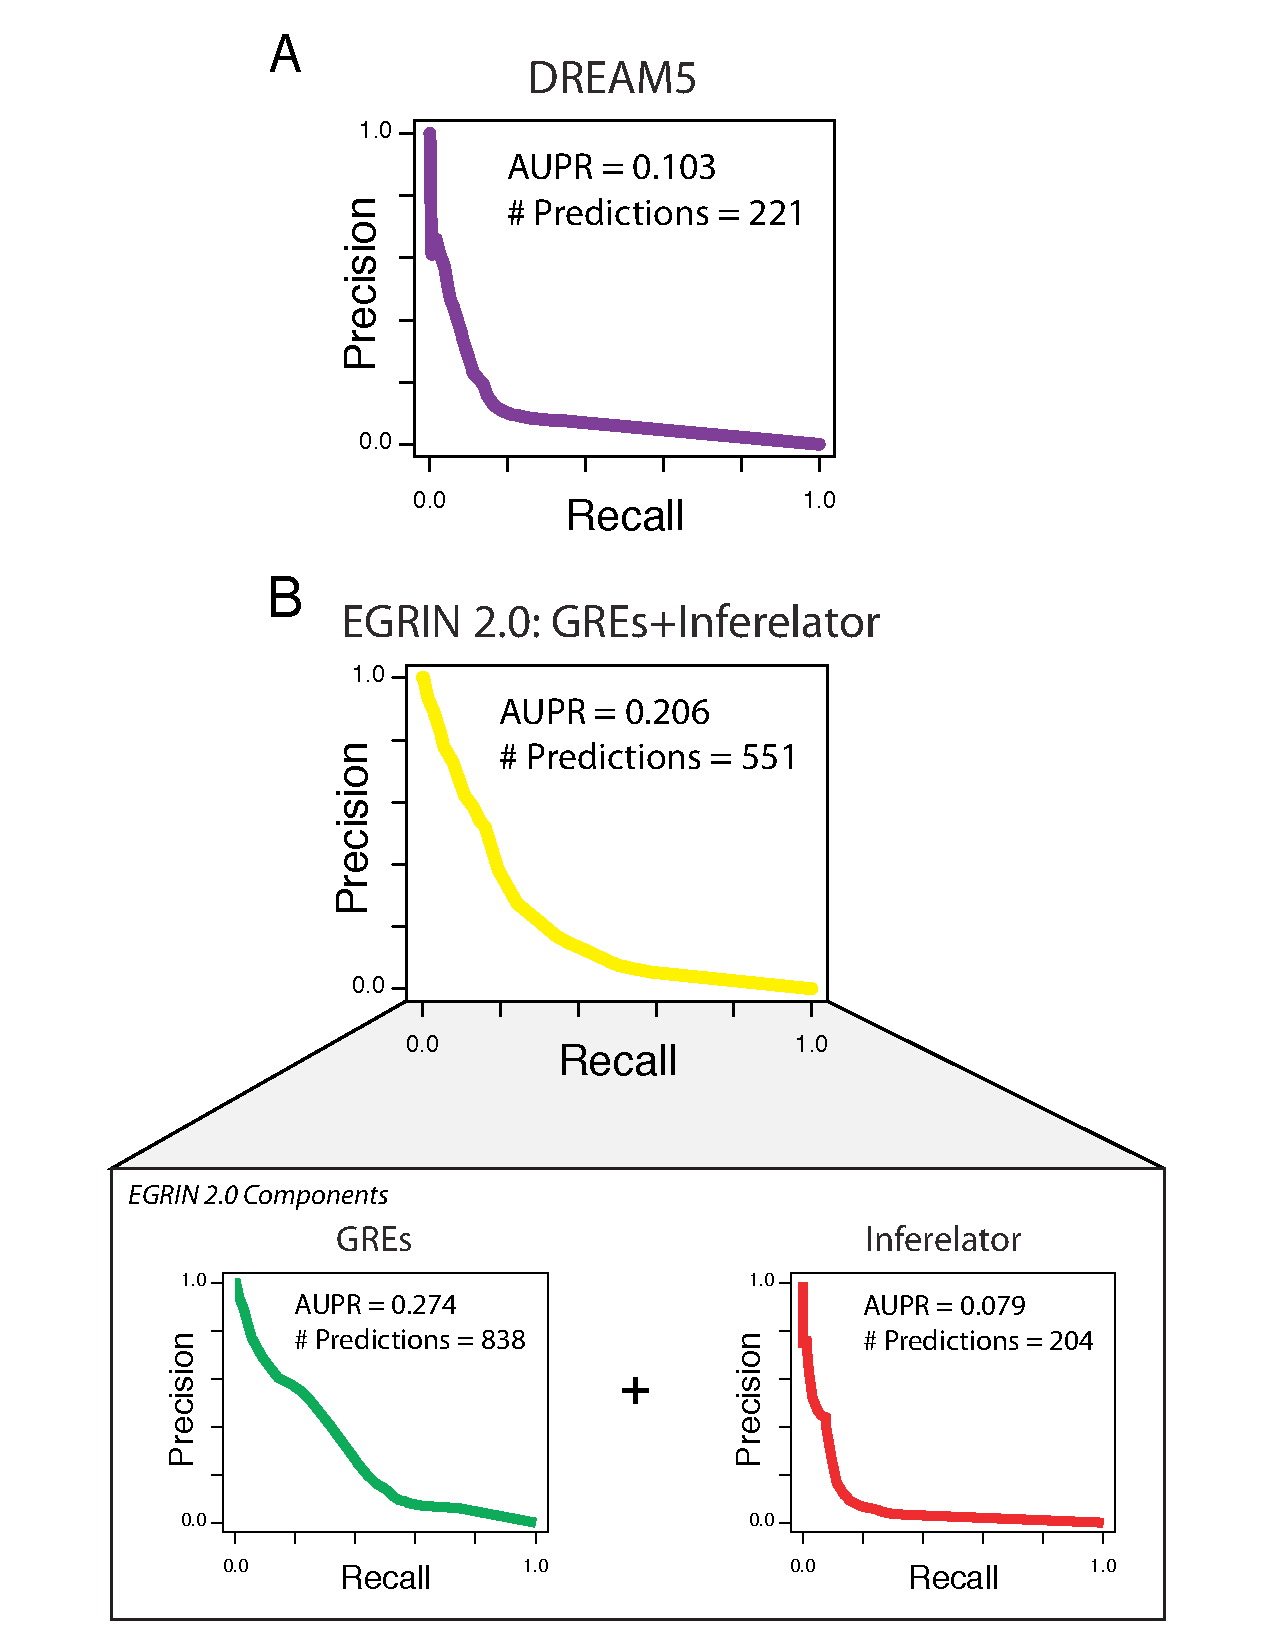
\includegraphics[width=0.5\linewidth]{figures/aupr.pdf}
\caption[Precision-recall performance for {\it E. coli} networks.]{\textbf{Precision-recall performance for \textit{E. coli} networks.} Comparison of precision-recall performance on {\it E. coli} \rdb~gold-standard (Section \ref{section:eco:gold:standard}), for the DREAM5 ensemble network (A), compared to \egrine (B).  We compare the GRE-based and \nwinf-based networks (bottom)to the integrated \egrine~network (top). The integrated \egrine~network consists of an equal weighting of the GRE-based and \nwinf-based networks.  The \egrine~networks were inferred using the DREAM5 mRNA expression compendium (Section \ref{section:dream5_data_compendium}). Area under the curve (AUPR) and the number of true-positive predictions at a precision of 25\% are listed for each curve.} 
\label{fig:pr_curves}
\end{figure}

We further investigated the convergence of the AUPR statistics for each of the \egrine-predicted regulatory networks as additional individual EGRIN models are added to the ensemble. This assessment helps to address the question of whether the approach utilized for ensemble integration has the desired property of performing better than most (if not all) of the individual models. Additionally, it can address the question of how many individual EGRIN models are necessary to achieve a given performance level. We observed that this is indeed the case for the \nwinf-based predictions extracted from the \egrine\ model (Figure~\ref{fig:cumulative_auprs}a), whose final AUPR of 8.5\% far exceeds the rather poor performance of all 106 individual component EGRIN models (with an average AUPR of 5.0\% and a maximum of 7.4\%). The performance of the ensemble for this measure converges rather quickly to the final measure, after roughly 50 of the 106 EGRIN models are integrated (taking into account the variance in models observed with integrating the models in different orders).  For the \egrine\ GRE-based predicted network (Figure~\ref{fig:cumulative_auprs}b), ensemble surpasses 84 (79\%) of the 106 individual component EGRIN models. This measure continues to improve until $\sim 80$ of the 106 models are integrated, suggesting that for this data set (the DREAM5 {\it E. coli} expression compendium), $\sim 100$ EGRIN models was a reasonable number to use in construction of the \egrine\ ensemble.

\begin{figure}[hp]
\centering
\mbox{
\subfigure[]{\includegraphics[width=0.4\linewidth]{figures/nwInf_cumulative_forPaper.pdf}}
\subfigure[]{\includegraphics[width=0.4\linewidth]{figures/motif_cumulative_forPaper.pdf}}
}
\caption[Ensemble performance of individual GRN predictions]{\textbf{Ensemble performance of individual GRN predictions.} \egrine-inferred \textit{E. coli} regulatory network predictive performance (AUPR vs. {\it E. coli} DREAM5 \cite{marbach_wisdom_2012} gold standard) for \nwinf-based predictions (a) and GRE-based predictions (b) from \egrine. Shown for both networks is the cumulative AUPR as each of the 106 individual model components is integrated in to the ensemble (as described in Section~\ref{section:aupr:vs:regdb}). Lines showing the cumulative AUPR for randomized orderings of the components' integration into the ensemble reveal the slight variations in performance that could be observed, and that these converge prior to integration of the final ($106^{\text{\tiny th}}$) component. Also included for comparison is a box-whisker plot which shows the distribution of corresponding AUPR scores for the 106 individual EGRIN models. } 
\label{fig:cumulative_auprs}
\end{figure} 

Figure \ref{fig:argR_purR_networks} shows the inferred networks for two genes regulated by PurR and ArgR (comparing predictions from \egrine, \tmsamp{CLR}, DREAM5, and \tmsamp{RegPrecise} to the annotations in \rdb). The result demonstrates that GRE-based approaches can discover interactions that are not predicted using direct approaches (See Section~\ref{section:gre_grn_construction}).

\begin{figure}[hp]
\centering
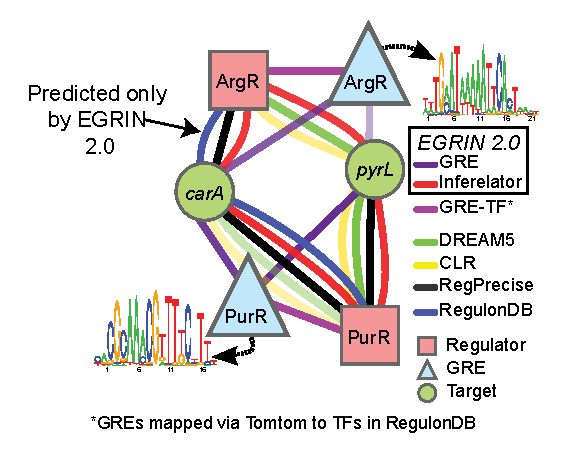
\includegraphics[width=0.5\linewidth]{figures/argR_purR_networks.pdf}
\caption[Integration of GRE discovery and \nwinf\ predictions yields comprehensive and detailed gene regulatory networks]{\textbf{Integration of GRE discovery and \nwinf\ predictions yields comprehensive and detailed gene regulatory networks.} \egrine-inferred \textit{E. coli} regulatory subnetwork for two genes (green circles) in the PurR/ArgR regulon: \textit{carA} (\textit{b0032}) and \textit{pyrL} (\textit{b4246}). The \egrine~predictions are divided into GRE-based (dark violet) and \nwinf-based (red), and compared to predictions (or annotations) from other algorithms/databases (yellow: \tmsamp{CLR}; green: DREAM5 ensemble; black: \tmsamp{RegPrecise}; blue: \tmsamp{RegulonDB}). In two cases (ArgR$\rightarrow$carA and ArgR$\rightarrow$pyrL), \egrine~discovers regulatory interactions that were missed by either hand-curated databases or expression-based inference procedures.} 
\label{fig:argR_purR_networks}
\end{figure} 

\subsection{Validation of condition-specific operon isoforms by tiling array transcriptome measurements}

We validated the prevalence of multiple, condition-specific transcriptional isoforms from operons in \eco\ by measuring changes in the transcriptome across growth, from lag-phase (OD600 = 0.05) to late stationary phase (OD600 = 7.3). The experimental platform and other experimental details are described in Section \ref{section:ecoarray}. We used multivariate recursive partitioning, including signals from both relative changes in expression along the growth curve, as well as raw RNA hybridization signal to call putative transcription breaks as previously described \cite{koide_prevalence_2009}. To determine the significance of our finding, we computed a $p$-value describing the significance of the overlap between our predictions (see Section \ref{section:condop}) and the experimental observations using the cumulative hypergeometric distribution.

Figures \ref{fig:dpp_ecoli_expression}, \ref{fig:galE}, and \ref{fig:ptsh} below depict several operons annotated with condition-specific transcriptional isoforms. We have integrated GRE elements discovered near break sites with the transcriptional measurements.

\begin{figure}[hp]
\centering
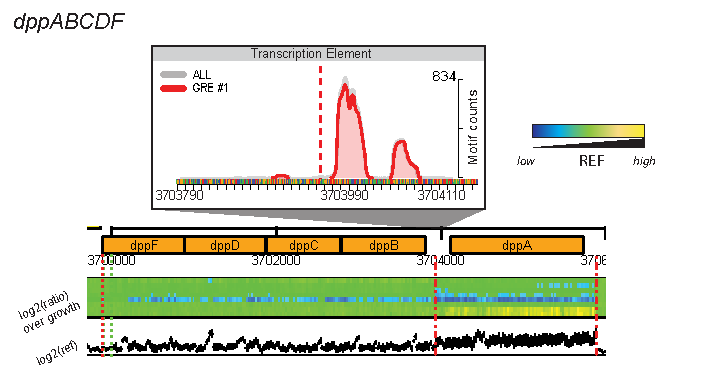
\includegraphics[width=0.7\linewidth]{figures/dpp_ecoli_expression.pdf}
\caption[GREs regulate multiple transcript isoforms from operons in {\it E. coli}, \textit{dppABCDF}]{\textbf{GREs regulate multiple transcript isoforms from operons in {\it E. coli}, \textit{dppABCDF}.} GREs coincide with experimentally measured break sites. Three examples of experimentally determined transcription break sites (red dashed lines) in operons predicted by corems to be conditionally segmented. Expression levels of these regions were profiled across growth in rich media (heatmap). Inset contains region immediately surrounding a transcriptional break site, including counts of GREs discovered at these locations.} 
\label{fig:dpp_ecoli_expression}
\end{figure}

\begin{figure}[hp]
\centering
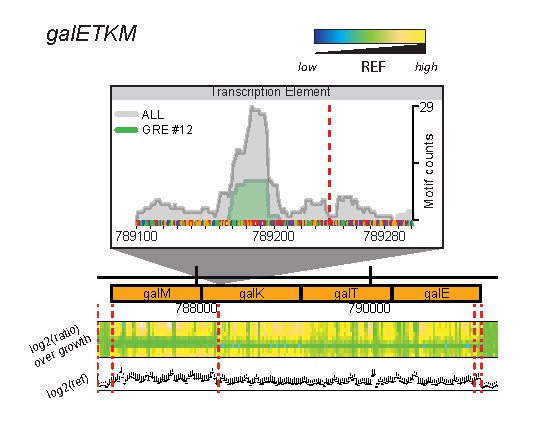
\includegraphics[width=0.7\linewidth]{figures/galE.pdf}
\caption[GREs regulate multiple transcript isoforms from operons in
  {\it E. coli}, \textit{galETKM}]{\textbf{GREs regulate multiple
    transcript isoforms from operons in {\it E. coli},
    \textit{galETKM}.} Caption details included in Figure
  \ref{fig:dpp_ecoli_expression}}
\label{fig:galE}
\end{figure}

\begin{figure}[hp]
\centering
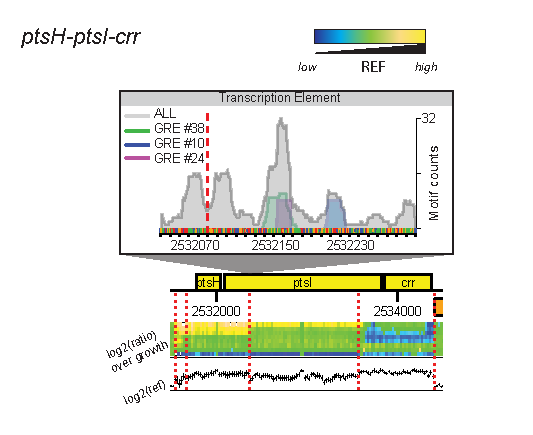
\includegraphics[width=0.7\linewidth]{figures/ptsh.pdf}
\caption[GREs regulate multiple transcript isoforms from operons in
  {\it E. coli}, \textit{ptsH-ptsI-crr}]{\textbf{GREs regulate
    multiple transcript isoforms from operons in {\it E. coli},
    \textit{ptsH-ptsI-crr}.} Caption details included in Figure
  \ref{fig:dpp_ecoli_expression}.}
\label{fig:ptsh}
\end{figure}

\subsection{Gene-gene co-fitness correlations in corems}

To assess the phenotypic consequences of co-regulation in corems, we assessed whether genes grouped into corems had significantly similar fitness consequences in many environments (\ie, the effect of deleting one gene is highly similar to the effect of deleting the other across many environments). We used the high-throughput fitness screen described in Section \ref{section:fitness} to quantify these relationships.

We compared the enrichment for high co-fitness relationships in corems to other ways of assigning co-regulatory modules, including regulons (\tmsamp{RegPrecise}, \rdb), operons, and \tmsamp{WGCNA}. The gene modules for regulons (annotated in \rdb\ or \tmsamp{RegPrecise} \cite{novichkov_regprecise_2012}) consisted of genes annotated to a common TF. For WGCNA, we assigned modules using the same community detection procedures that we used to define corems from the \egrine~ensemble (See \ref{section:gBg}). The gene co-expression modules were computed from the weighted \tmsamp{WGCNA} adjacency matrix.

For the results presented in Figure~\ref{fig:egrin2:2:B}, we compared the distributions of Pearson correlations between relative changes in fitness across pairs of genes within each module, using the one-tailed Kolmogorov-Smirnov test (KS-test). We report the KS $D$-statistic. The precision/recall characteristics for each model are contained in Table~S5.

We extended this analysis by investigating whether the enriched high co-fitness gene-gene relationships in corems consist of relationships that could be described fully by regulons or operons. To answer this question, we removed all gene pairs from corems that are also present in operons or regulons and computed the KS-test again (Figure \ref{fig:fitness_wo_operons}). We still observe a significant number of high co-fitness relationships, suggesting that corems capture physiologically meaningful co-regulatory relationships between genes that cannot be explained by existing paradigms.

\begin{figure}[hp]
\centering
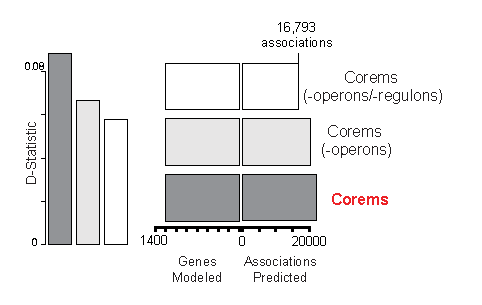
\includegraphics[width=0.6\linewidth]{figures/fitness_wo_operons.pdf}
\caption[\egrine~models highly correlated co-fitness relationships that cannot be explained by operons or regulons]{\textbf{\egrine~models highly correlated co-fitness relationships that cannot be explained by operons or regulons.} (Left) Enrichment for highly correlated, pairwise fitness measurements in gene knock outs across 324 conditions before and after removing gene associations annotated by operons (Microbes Online) and regulons (RegulonDB and RegPrecise) (KS-test,$D$-statistic). Two-thirds of gene-pairs with most highly correlated fitness within corems are not annotated by operons or regulons. (Right) Number of genes and associations predicted.} 
\label{fig:fitness_wo_operons}
\end{figure}



 

 
 